\documentclass[xcolor=dvipsnames]{beamer}
\usetheme{nelle}
\usepackage{natbib}                 % Fancy bibliography.
\usepackage{url}                    % Allow printing of URLs.
\usepackage{outlines}
\usepackage{enumitem}
\usepackage{multicol}
\usepackage{dsfont}
\usepackage{amsmath}
\usepackage{epstopdf}
\usepackage{color}
\setbeamerfont{caption}{size=\scriptsize}
\setbeamertemplate{navigation symbols}{}
\setbeamertemplate{footline}[frame number]{}

\def\newblock{\hskip .11em plus .33em minus .07em}

\title{\textbf{Inferring the 3D structure of the genome}}

\author[Varoquaux Nelle]{
Nelle Varoquaux}


\date{December, 3rd}
\institute{Mines ParisTech, Institut Curie, INSERM}
\begin{document}
\begin{frame}[t, noframenumbering]
  \maketitle

\end{frame}

\setcounter{framenumber}{0}

\section{Introduction}
% 1. Why?
\begin{frame}
\frametitle{The 3D structure of the genome is thought to play an important
role in many biological processes}
\vspace{-0.6em}
\begin{figure}
\begin{center}
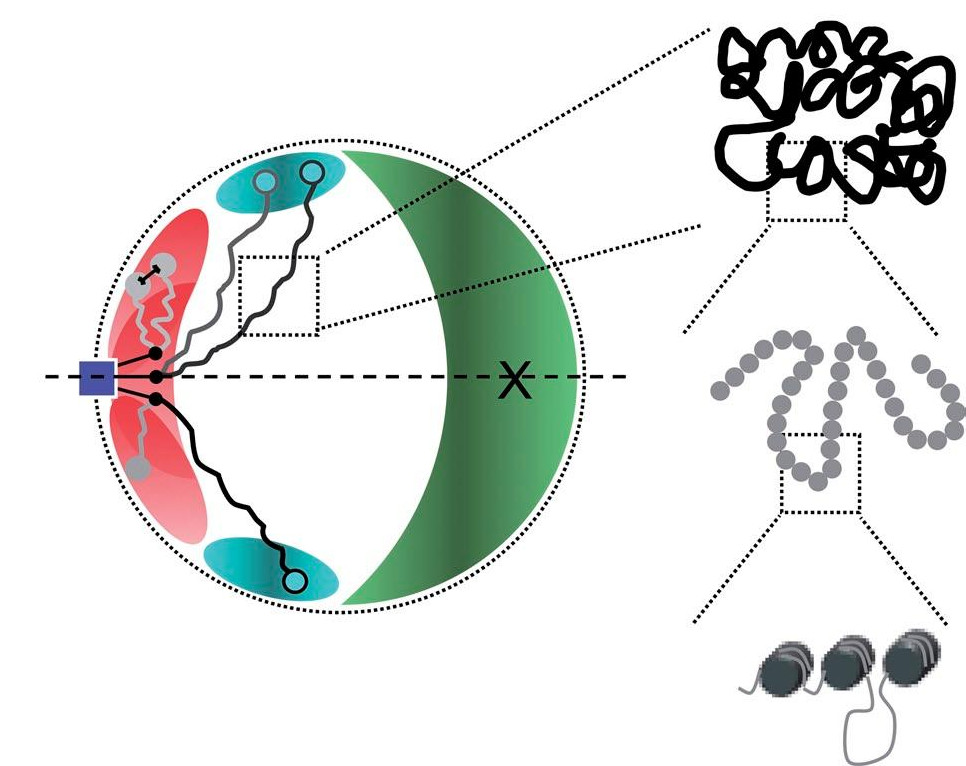
\includegraphics[width=0.7\linewidth]{figures/yeasts_genome_architecture.jpg}
\end{center}
\caption{\textbf{The genome of \textit{S. cerevisiae} is highly organized}
         \citep{zimmer:principles}}
\end{figure}
\end{frame}

% 2. What is the Hi-C protocol?
\begin{frame}
\frametitle{The Hi-C protocol identifies physical contacts between
pairs of loci genome-wide}
\begin{figure}
\centering
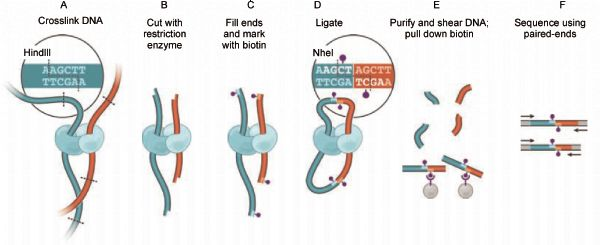
\includegraphics[width=0.85\textwidth]{figures/hic_protocol.jpg}
\caption{\textbf{Hi-C paves the way for a systematic and genome-wide analysis
of genome architecture} \citep{rao:3d}}
\end{figure}
\end{frame}

% 3. A contact count matrix
\begin{frame}
\frametitle{The contact count matrix recapitulates the hallmarks of genome
architecture}
\vspace{-1em}
\begin{figure}
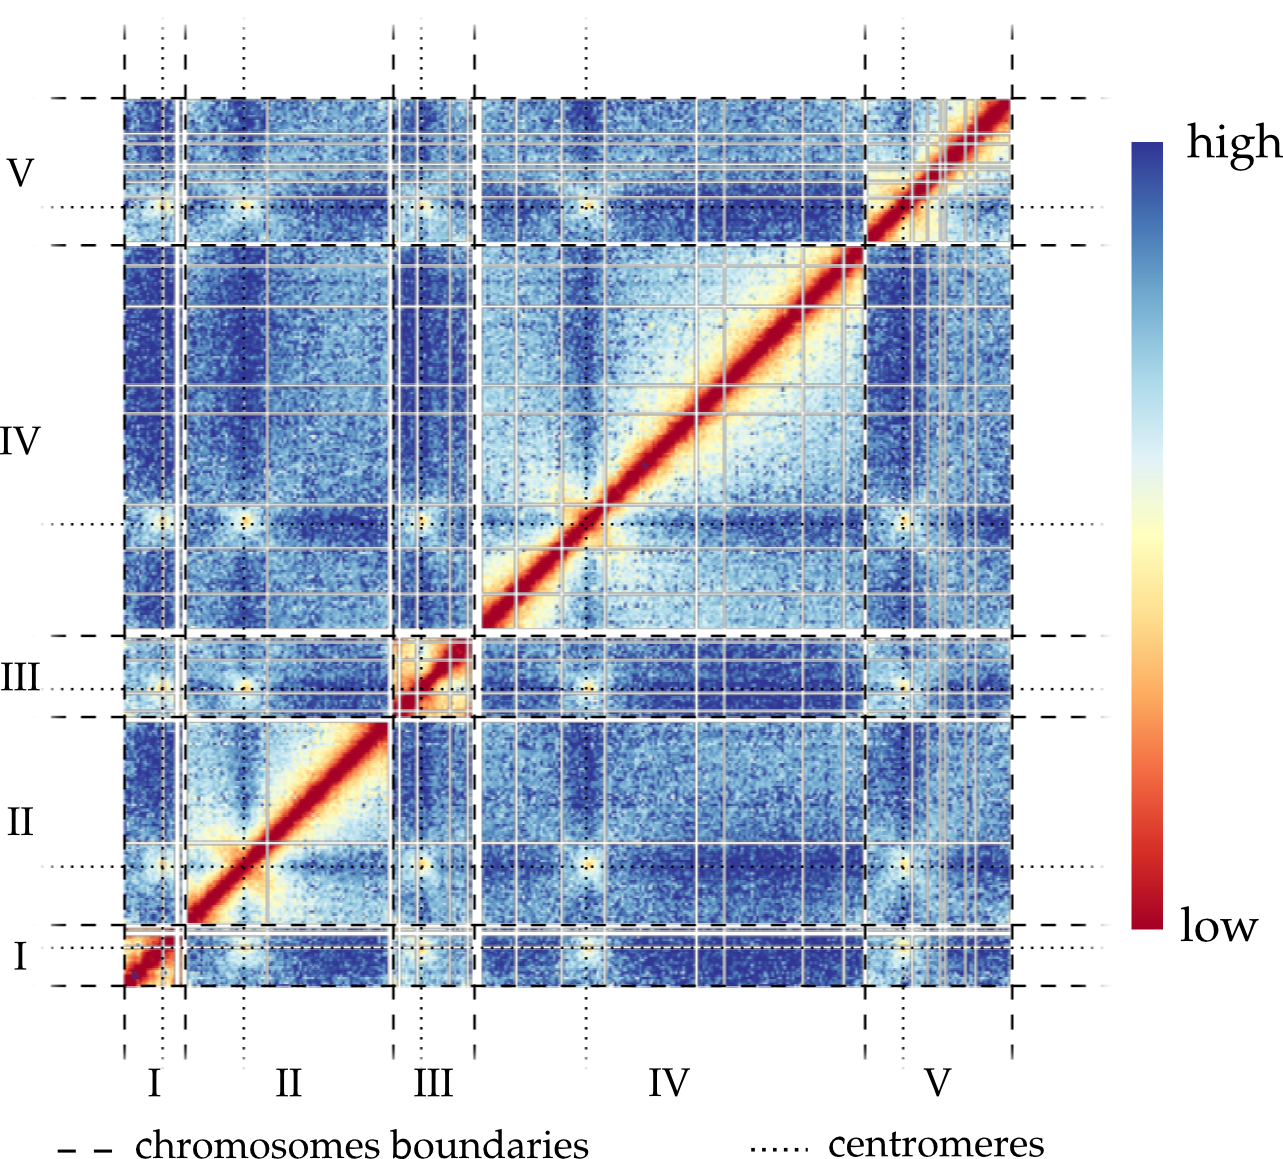
\includegraphics[width=0.55\textwidth]{figures/yeast_counts.pdf}
\caption{\textbf{Contact counts for the first 5 chromosomes of \textit{S.
cerevisiae}}}
\end{figure}
\end{frame}

\begin{frame}
\frametitle{HiC-Pro: from sequences to contact maps}
\begin{figure}
\begin{center}
\includegraphics[width=0.9\linewidth]{figures/hic-pro.pdf}
\end{center}
\end{figure}
\end{frame}

\begin{frame}
\frametitle{A wide range of applications for Hi-C data}
\begin{overlayarea}{12cm}{6cm}
\begin{itemize}
\item<1-> \textbf{Studying the 3D structure of the genome}: 3D structure
inference, data integration with gene expression profiles, replication timing,
\dots
\item<2-> \textbf{Studying the 1D structure of the genome}: genome assembly,
metagenomic deconvolution, haplotype resolution, \dots
\item<3-> \textbf{Genome annotation}: identifying rDNA clusters, centromeres,
specific gene families, \dots
\end{itemize}
\end{overlayarea}
\begin{overlayarea}{12cm}{3cm}
\only<1>{
\vspace{-4cm}
\begin{center}
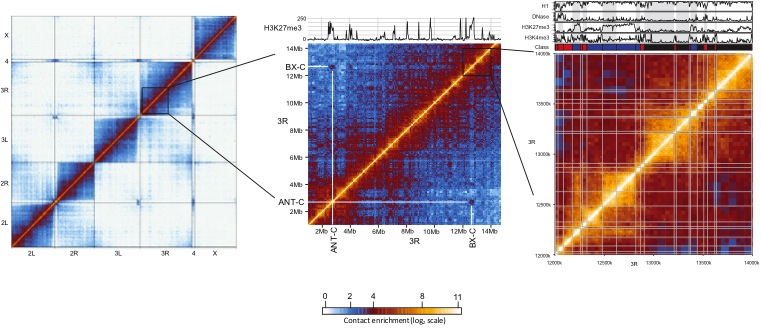
\includegraphics[width=0.9\linewidth]{figures/cavalli-illustration.jpg}
\end{center}}
\only<2>{
\vspace{-4cm}
\begin{center}
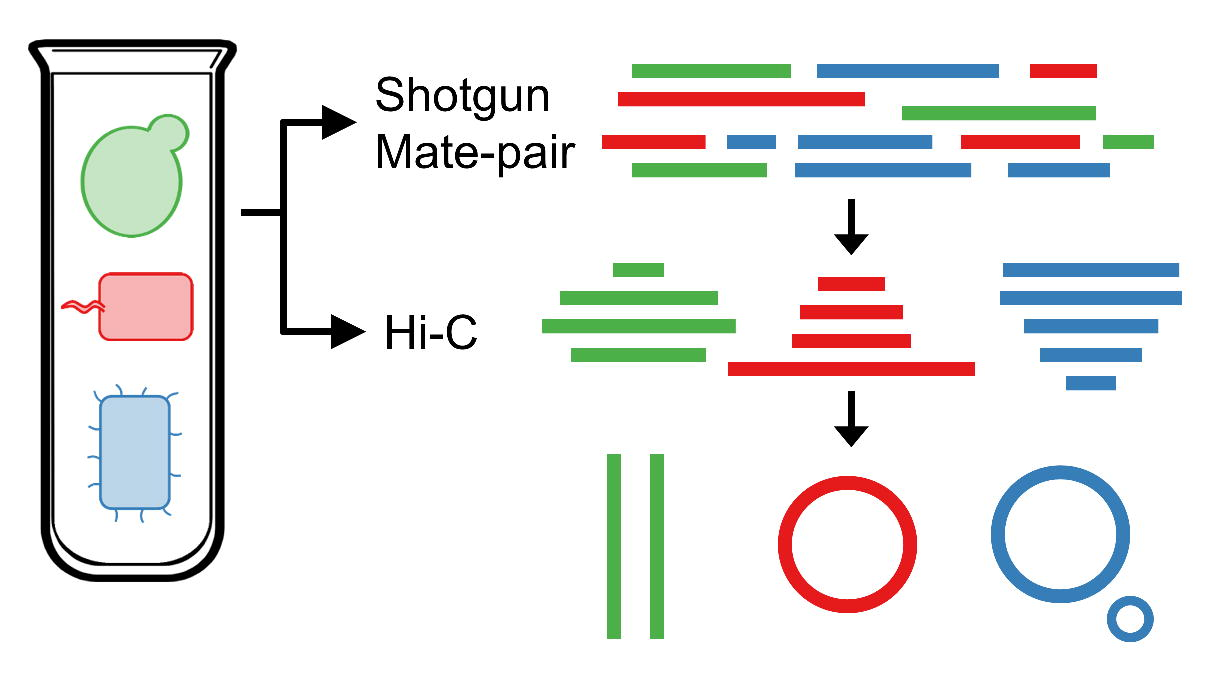
\includegraphics[width=0.75\linewidth]{figures/metagenomic_deconvolution.png}
\end{center}}
\only<3>{
\vspace{-3cm}
\begin{center}
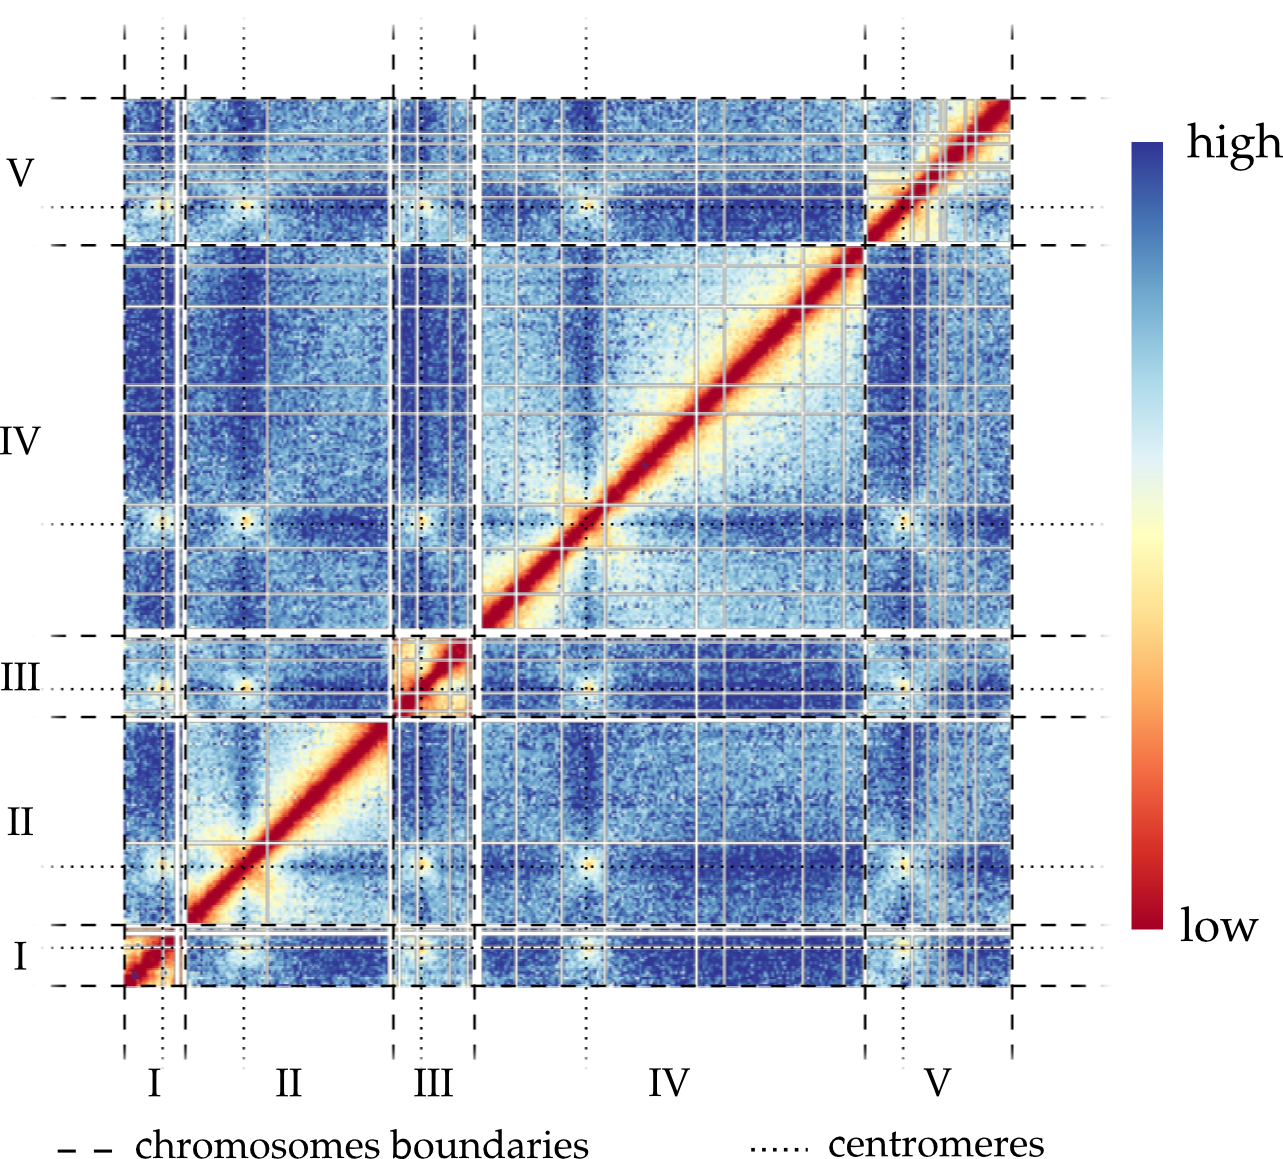
\includegraphics[width=0.45\textwidth]{figures/yeast_counts.pdf}
\end{center}}
\end{overlayarea}
\end{frame}

\begin{frame}
\frametitle{Contributions}
\begin{itemize}[label={$\bullet$}]
\item<1-> A statistical approach for inferring the 3D structure of the
genome. \textit{Bioinformatics, 2014}
\item<2-> Three-dimensional modeling of the {\em P. falciparum} during the
erythrocytic cycle reveals a strong connection between genome architecture and
gene expression. \textit{Genome Research, 2014}
\item<3-> Accurate identification of centromere locations in yeast genomes using
Hi-C. \textit{Nucleic Acids Research, 2015}
\end{itemize}

\begin{itemize}[label={$\circ$}]
\item<4-> HiC-pro: An optimized and flexible pipeline for Hi-C data
processing. \textit{Genome Biology, 2015}
\item<5-> Identifying multi-locus chromatin contacts in human cells using teth-
ered multiple 3C. \textit{BMC Genomics, 2015}
\item<6-> Multiple dimensions of epigenetic gene regulation in the malaria
parasite {\em Plasmodium falciparum}.
\textit{Bioessays, 2015}
\end{itemize}
\end{frame}





\section{A statistical approach for inferring the 3D structure of the genome}

\begin{frame}
\Large{ \bf
A statistical approach for inferring the 3D structure of the genome.}

\begin{flushright}
\vspace{1em}
\small
\textit{joint work with 
Ferhat Ay, William S. Noble \\ and Jean-Philippe Vert.}
\end{flushright}
\end{frame}

% 1. Motivation
\begin{frame}
\frametitle{Inferring 3D models of genome architecture from Hi-C data}
{\color{Blue} \textbf{Motivation}}
\begin{itemize}[label={$\bullet$}]
\item Little is known on the 3D structure of the genome.
\item Hi-C now allows to assess physical interactions genome-wide.
\end{itemize}

\vspace{1em}
{\color{Blue} \textbf{Goal}} Propose a robust and accurate method for
inferring 3D models of genome architecture from contact counts.

\vspace{1em}
{\color{Blue} \textbf{Idea}} Model contact counts as Poisson random variables
where the 3D model is a latent variable and cast the inference as maximizing
the likelihood.

\end{frame}

% 2. Consensus vs Population based model

\begin{frame}
\frametitle{Reconstructing the 3D structure from contact counts maps}
\begin{columns}
\begin{column}{0.5\textwidth}
\begin{center}
{\large \textbf{Consensus approach}}
\end{center}
\begin{figure}
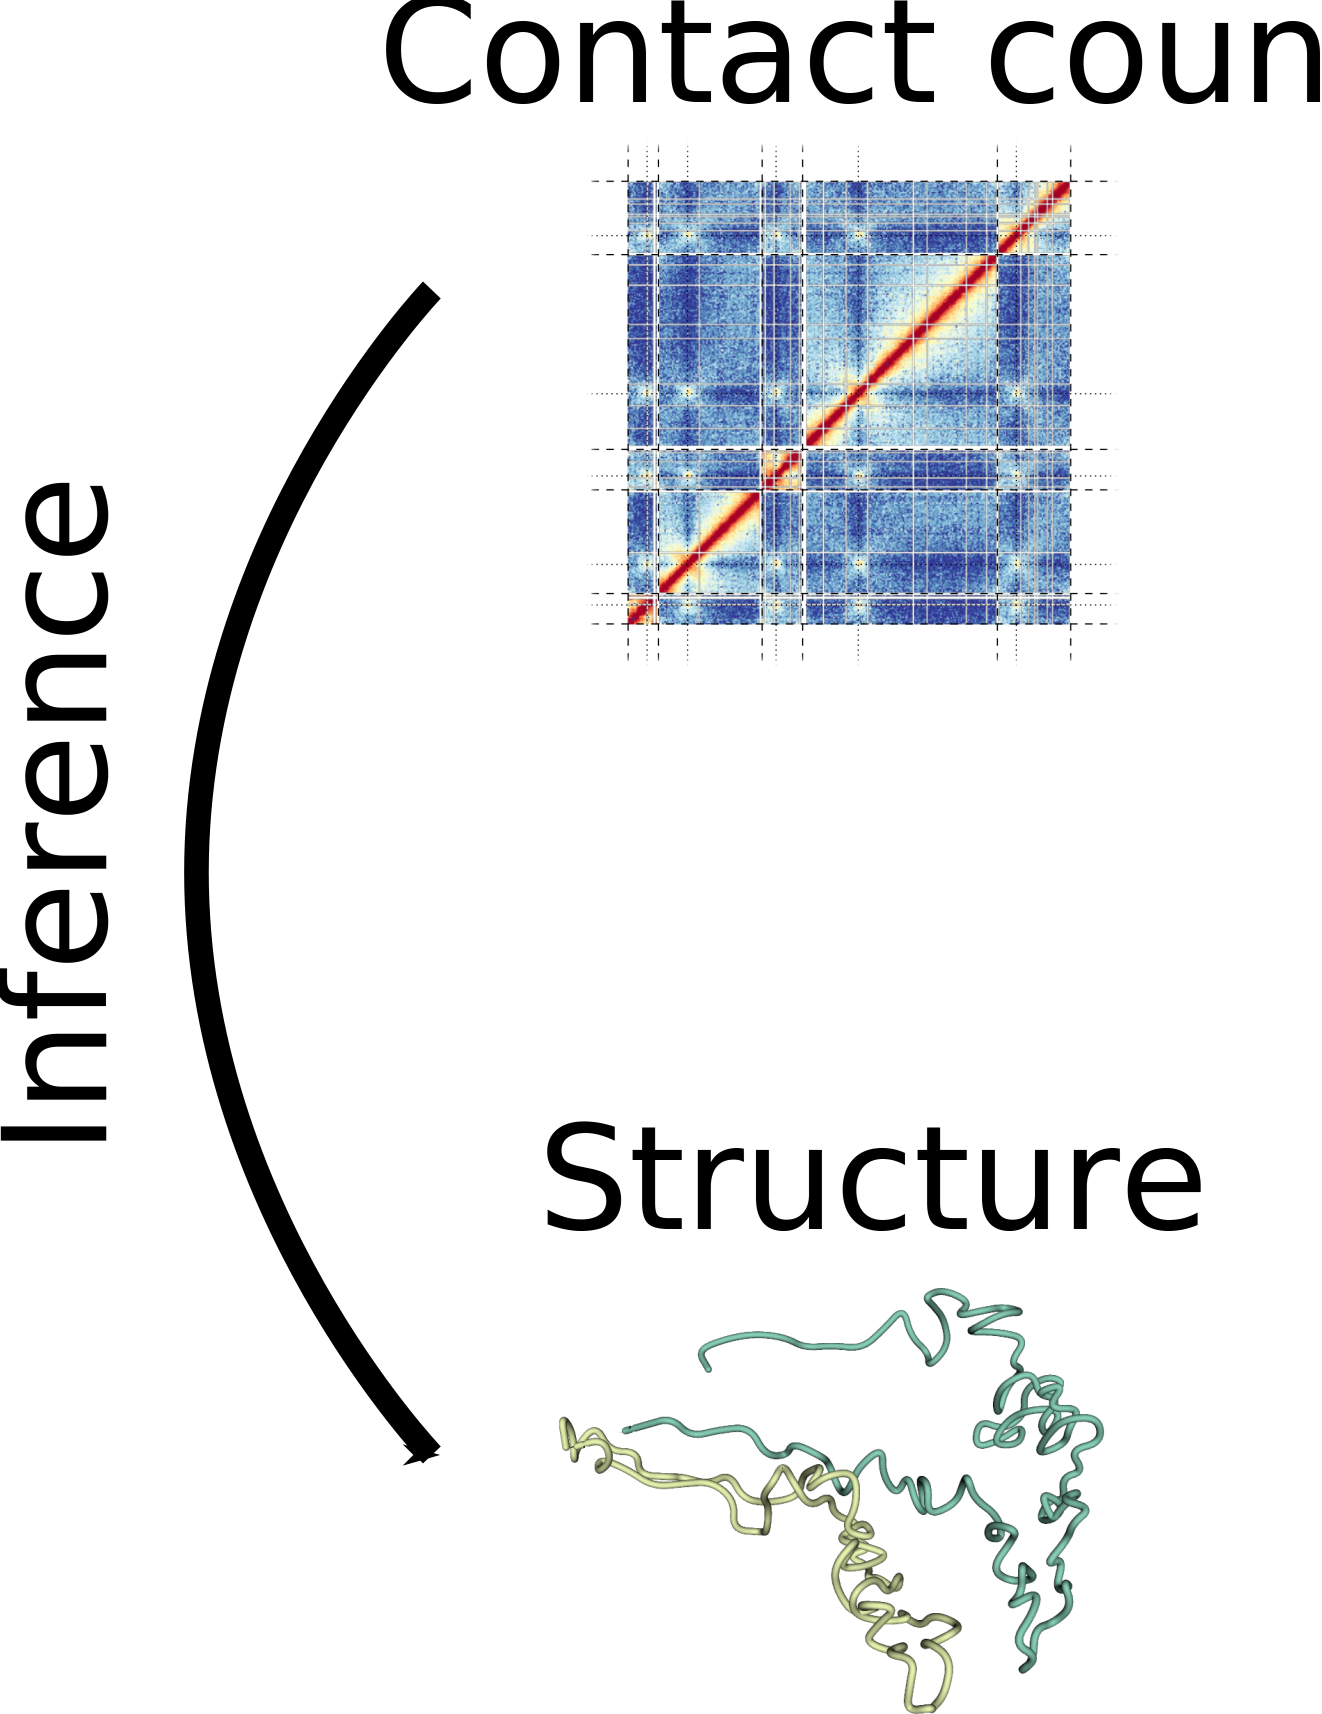
\includegraphics[width=0.6\textwidth]{figures/inference_mean_structure.pdf}
\end{figure}
{\tiny \citep{duan:three-dimensional, tanizawa:mapping,
bau:three-dimensional, zhang:inference, ben-elazar:spatial,
lesne:3d}}
\end{column}
\begin{column}{0.5\textwidth}
\begin{center}
{\large \textbf{Ensemble approach}}
\end{center}
\begin{figure}
\includegraphics[width=0.6\textwidth]{figures/inference_population_structure.pdf}
\end{figure}
{\tiny
\citep{rousseau:three, hu:bayesian, kalhor:genome, tjong:physical}}
\end{column}
\end{columns}
\end{frame}

% 3. Notation
\begin{frame}
\frametitle{Chromosomes as a series of beads}

\begin{figure}
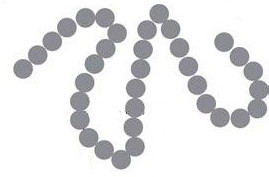
\includegraphics[width=0.25\linewidth]{figures/chrom_as_series_beads.jpg}
\end{figure}

\begin{itemize}[label={$\bullet$}]

\item Let $\mathbf{X} \in R^{n \times 3}$ be the coordinates of each bead.
\item Let $\mathbf{C} \in R^{n \times n}$ be the raw contact count matrix.
\item Let $\Theta$ the count-to-distance transfer function.
\end{itemize}

\vspace{2em}
{\color{Blue} \bf Optimization problem}
\begin{equation*}
\renewcommand{\arraystretch}{2}
\begin{array}{ccll}
\underset{{\bf x}_1,\ldots,{\bf x}_n}{\text{minimize}} & &
\sigma(\mathbf{X}, \mathbf{C})\\
\end{array}
\end{equation*}
\end{frame}


\begin{frame}
\frametitle{Relationships between contact counts $c$, genomic distances $s$
and Euclidean distances $d$}
\begin{columns}
\begin{column}{0.5\textwidth}
\begin{center}
\textbf{Fractal globule}
\begin{figure}
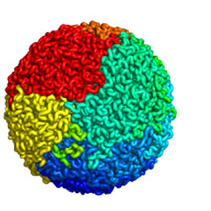
\includegraphics[scale=0.3]{figures/mirny_fractal.png}
\end{figure}
\end{center}
\begin{itemize}[label={$\bullet$}]
  \item $c \sim s^{-1}$
  \item $d \sim s^{1 / 3}$
\end{itemize}
\end{column}

\begin{column}{0.5\textwidth}
\begin{center}
\textbf{Equilibrium}
\begin{figure}
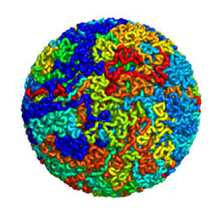
\includegraphics[scale=0.3]{figures/mirny_equilibrium.png}
\end{figure}
\end{center}
\begin{itemize}[label={$\bullet$}]
  \item $c \sim s^{-3 / 2}$
  \item $d \sim s^{ 1 / 2} \quad \text{for} \quad s < s_{\text{max}}^{2 / 3}$
\end{itemize}
\end{column}
\end{columns}

\vspace{2em}
{\bf \color{Blue} Relationship between contact counts and Euclidean distances}
\\
\begin{equation*}
d_{ij} = \gamma c_{ij} ^{-1/3},
\end{equation*}


\end{frame}

% 4. MDS

\begin{frame}
\frametitle{Metric MDS-based methods}

\begin{figure}
\begin{center}
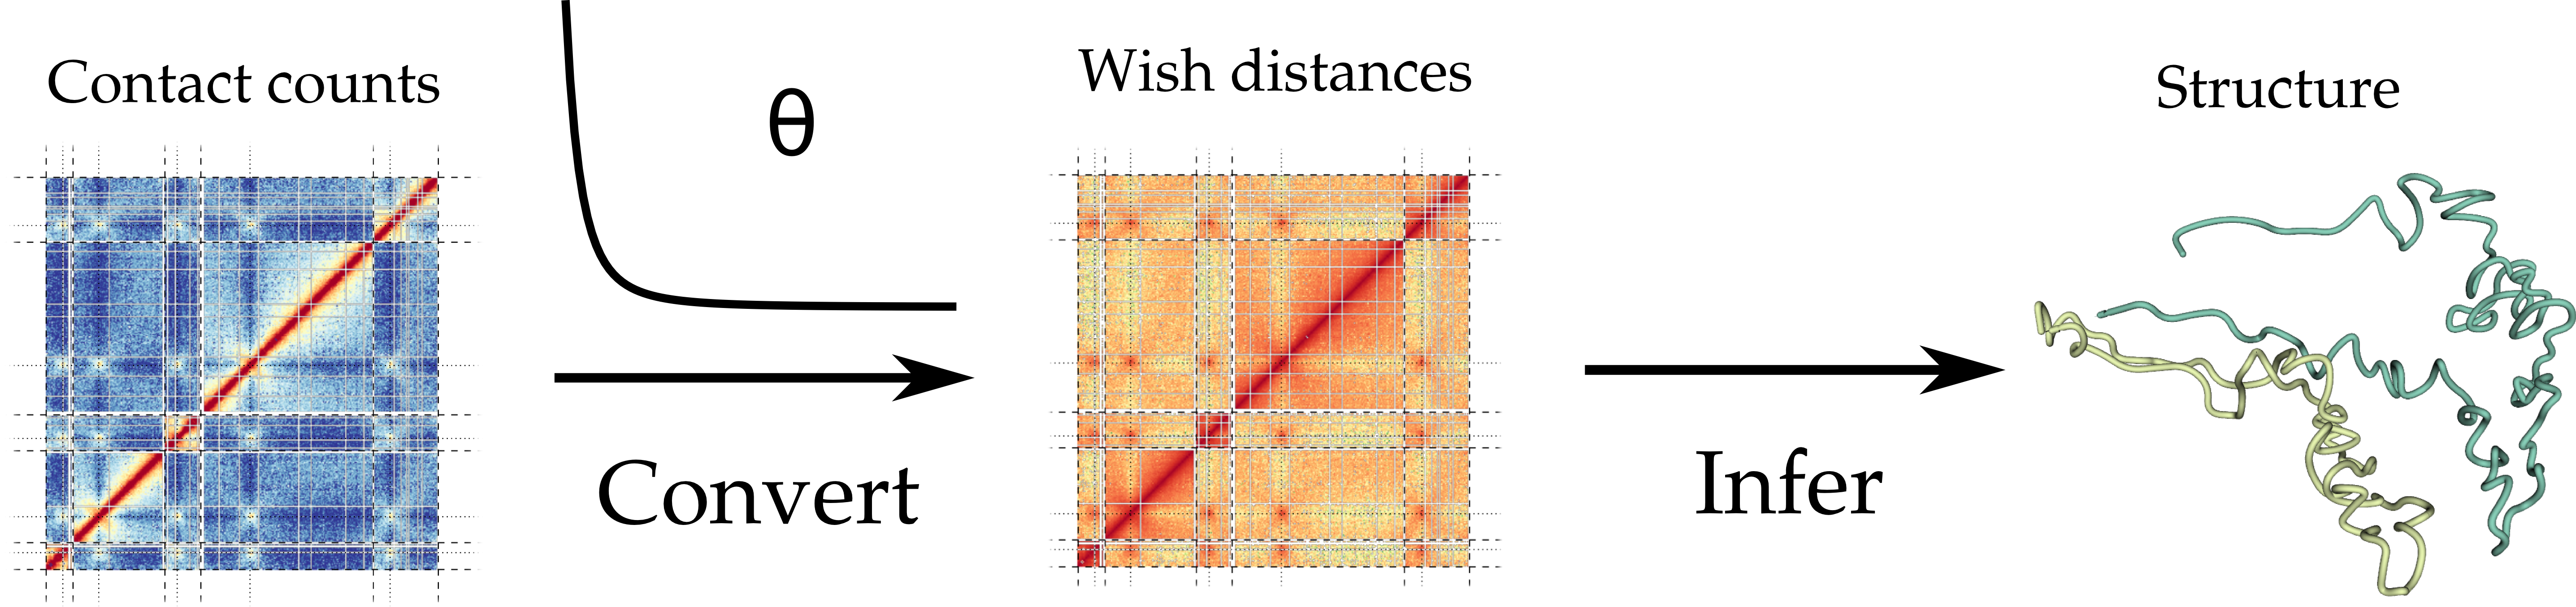
\includegraphics[width=0.9\linewidth]{figures/mds_idea.png}
\end{center}
\end{figure}
\vspace{1em}

\textbf{\color{Blue} Formulation}
\begin{equation*}
\renewcommand{\arraystretch}{2}
\begin{array}{ccll}
\underset{{\bf x}_1,\ldots,{\bf x}_n}{\text{minimize}} & &
\sigma(\mathbf{X},  C) = \underset{i, j | c_{ij} \neq 0}{\sum} w_{ij}(\|x_i - x_j\|_2 -
\Theta(c_{ij}))^2\,
\\
\end{array}
\end{equation*}
\vspace{2em}

{\tiny
\begin{multicols}{2}
\begin{itemize}[label={$\bullet$}]
\item $\mathbf{X}$ : 3D coordinates
\item $\mathbf{C}$ : normalized contact counts.
\item $w_{ij}$ are weights (set to $\frac{1}{\Theta(c^N_{ij})^2}$ in
\textit{pastis-}\textbf{MDS2}) 
\item $\Theta(c) = \beta c^\alpha$: count-to-distance function
\end{itemize}
\end{multicols}
}
\end{frame}

\begin{frame}
\frametitle{Statistical approaches for inferring the 3D structure of the
genome}
\begin{itemize}[label={$\bullet$}]

\item MDS-based methods minimize an arbitrary stress function that measures
the discrepancy between wish distances and 3D distances of the model.
\end{itemize}

\vspace{1em}

{\color{Blue} \textbf{Statistical approach for stable inference of genome
structure}} \\
\begin{itemize}[label={$\bullet$}]

\item replace the arbitrary MDS loss function with a better-motivated
likelihood function
\item define a probabilistic model of contact counts parametrized by the 3D
model.
\end{itemize}
\end{frame}


% 5. The model

\begin{frame}
\frametitle{A Poisson model for inferring the 3D structure of the genome}
{\color{Blue} \textbf{The idea}} \\
Let's assume that $c_{ij} \sim Poisson(\beta d_{ij}^\alpha)$, where
$c_{ij}$ is the
interaction count, $d_{ij}$ the pairwise Euclidean distance, and $\beta$ and
$\alpha$
unknown parameters.
\vskip 1em

{\color{Blue} \textbf{Likelihood}}
\begin{equation*}
\ell(\mathbf{X}, \alpha, \beta) = \underset{i<j\leq n}{\prod} \frac{(\beta
d_{ij} ^\alpha)^{c_{ij}}}{c_{ij}!} exp(- \beta d_{j}^\alpha)
\end{equation*}
\vskip 1em
{\color{Blue} \textbf{Optimization problem}}
\vskip -2em
\begin{equation*}
\renewcommand{\arraystretch}{2}
\begin{array}{ccll}
\underset{{\bf x}_1,\ldots,{\bf x}_n, \alpha, \beta}{\text{minimize}} & &
\sigma(\mathbf{X}, \mathbf{C}, \alpha, \beta) = - \text{log}(\ell(\textbf{X},
\textbf{C}, \alpha, \beta)) \\
\end{array}
\end{equation*}
\end{frame}


% 6. The results on simulated data

\begin{frame}
\frametitle{Comparing methods}

{\color{Blue} \textbf{Methods}}: \textbf{MDS1}, \textbf{MDS2}, \textbf{NMDS},
\textbf{ChromSDE},
\textbf{PM1} (providing the parameter $\alpha$ using prior knowledge)
and \textbf{PM2} (inferring the parameters jointly with the structure) \\

\vspace{1em}
{\color{Blue} \textbf{Simulated Datasets}}
\begin{equation*}\label{eq:simu}
c_{ij} = \text{Poisson}(\beta d_{ij}^\alpha),
\end{equation*}
where 
\begin{itemize}[label={$\bullet$}]

\item $\alpha = -3$ and $\beta$ varies between 0.01 and 0.7.

\end{itemize}

\vspace{1em}
{\color{Blue} \textbf{Publicly available datasets}} mouse embryonic stem cells at
100~kb, 200~kb, 500~kb, 1~Mb {\scriptsize \citep{dixon:topological}},
normalized using ICE {\scriptsize
\citep{imakaev:iterative}}

\end{frame}



% 7. The results on real data

\begin{frame}
\frametitle{The Poisson models outperform MDS-based methods}
\begin{figure}
\includegraphics[width=0.8\textwidth]{figures/figure_slides_rmsd.pdf}
\end{figure}
\end{frame}

\begin{frame}
\frametitle{PM2 infers the most stable structures across different datasets}

{\scriptsize
\begin{table}
\begin{center}
\begin{tabular}{c | cc | cc | cc| cc}
\hline
Resolution & \multicolumn{2}{c}{1~Mb} & \multicolumn{2}{c}{500~kb} &
\multicolumn{2}{c}{200~kb} & \multicolumn{2}{c}{100~kb} \\
\hline
      &  RMSD & Corr  & RMSD  & Corr  & RMSD & Corr  & RMSD & Corr \\
\hline
MDS1  & 13.13 & 0.945 & 10.00 & 0.942 & 5.64 & 0.940 & 5.07 & 0.736 \\ 
MDS2  & 5.54  & 0.964 & 5.68  & 0.959 & 3.74 & 0.945 & 2.53 & 0.676 \\
NMDS  & 5.80  & 0.965 & 5.67  & 0.959 & 3.73 & 0.946 & 2.52 & 0.666 \\
PM1   & 7.28  & 0.931 & 7.14  & 0.913 & 4.01 & 0.891 & \textbf{2.51} & 0.664
\\
PM2   & \textbf{4.92} & \textbf{0.976} & \textbf{4.66} & \textbf{0.968} &
\textbf{3.42} & \textbf{0.958} & 2.76 & \textbf{0.771} \\
\hline
\end{tabular}
\end{center}
\caption{Average pairwise RMDS and correlation between structures inferred
from enzyme replicates datasets}
\end{table}
}
\end{frame}

% 8. Conclusion
\begin{frame}
\frametitle{Conclusion}
\begin{itemize}[label={$\bullet$}]

\item The Poisson model based methods outperform MDS-based methods.
\item Yet, the approach remains basic and could be subject to improvements:
  \begin{itemize}[label={$\bullet$}]

    \item better model for zero entries
    \item physical constraints
    \item diploid genome
  \end{itemize}
\end{itemize}

\vspace{3em}
{\footnotesize
The code for the Poisson Model is available online at
\url{http://cbio.ensmp.fr/pastis}.
}
\begin{figure}

\includegraphics[width=0.6\textwidth]{figures/pastis_logo.png}
\end{figure}
\end{frame}

\section{Three-dimensional modeling of the {\em P. falciparum} genome
during the erythrocytic cycle reveals a strong connection between genome
architecture and gene expression}

\begin{frame}

\Large{ \bf
Three-dimensional modeling of the \textit{P. falciparum} genome
during the erythrocytic cycle reveals a strong connection between genome
architecture and gene expression.}

\begin{flushright}
\vspace{1em}
\small
\textit{joint work with 
Evelien Bunnik, Ferhat Ay, \\
Sebastiaan Bol, Jacques Prudhomme, Jean-Philippe Vert, \\ William S. Noble and Karine
Le Roch.}
\end{flushright}

\end{frame}

% 1. Brief introduction of the P. falciparum
\begin{frame}
\frametitle{The human malaria parasite {\em P. falciparum}}

\begin{figure}
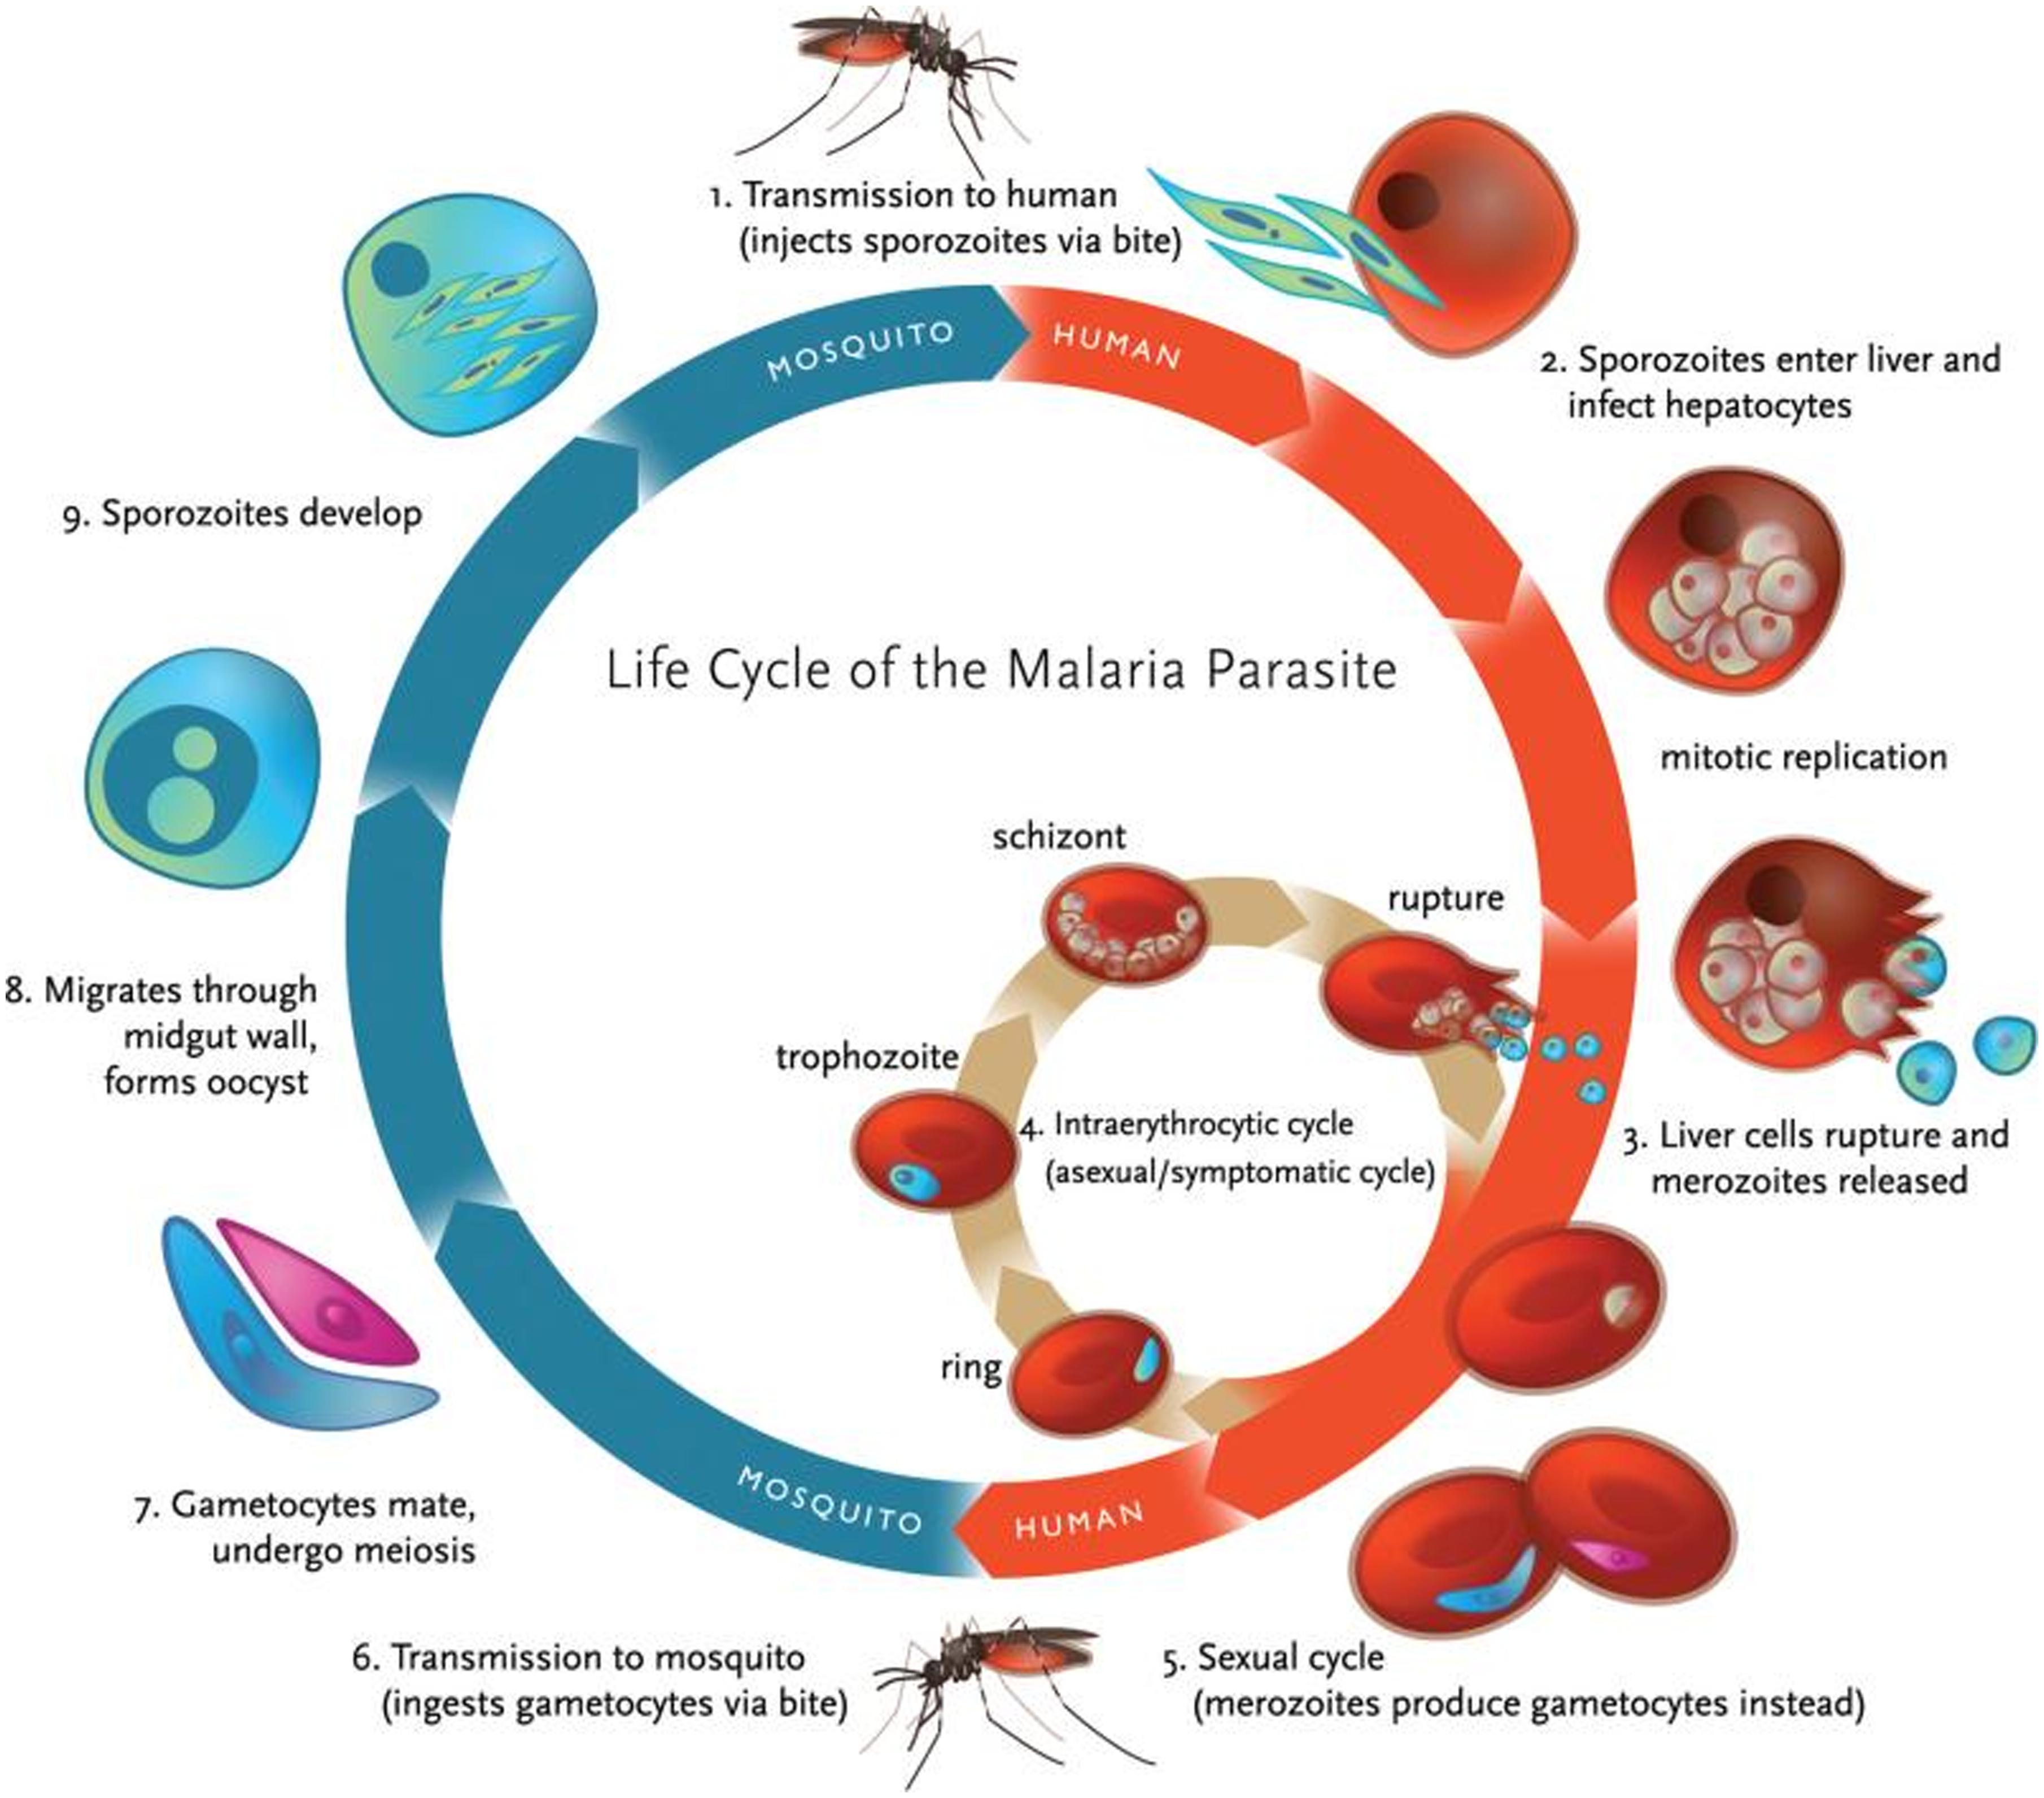
\includegraphics[width=0.75\linewidth]{figures/plasmodium_lifecycle.jpg}
\end{figure}
\end{frame}

% 2. Motivation and experiments
\begin{frame}
\frametitle{How are {\em P. falciparum's} gene expression and 3D structure related?}
{\color{Blue} \textbf{Motivation}}
\begin{itemize}[label={$\bullet$}]

\item One of the main limiting factors for the
development of therapies is the poor understanding of complex gene regulation
of the parasite.
\item The 3D architecture is thought to play an important role in gene
regulation.
\end{itemize}

\vspace{1em}
{\color{Blue} \textbf{Question}} How is the 3D structure of the genome related
to gene expression and regulation?

\vspace{1em}
{\color{Blue} \textbf{Experiment}} We performed Hi-C experiments at three time
points in the lifecycle of the parasite (ring, schizont and trophozoite
stages)

\end{frame}

% 3. 3D modeling
\begin{frame}
\frametitle{We inferred high resolution models of genome architecture at 3
timepoints}
\begin{figure}
\begin{equation*}
\renewcommand{\arraystretch}{2}
\begin{array}{ccll}
\underset{\mathbf{X}}{\text{minimize}} & &
\underset{c_{ij} \in \mathcal{D}}{\sum}
\frac{1}{\Theta(c_{ij})^2}\big(\|x_i - x_j\|_2 - \Theta(c_{ij})\big)^2 &\\
\text{subject to}
& & \|x_i\|_2^2 \leq r_{\rm max}^2, \quad
& i = 1:n\\
& & \|x_i - x_{i+1}\|_2 \leq b^{\rm max} , \quad
& i = \{1:n \;|\; {\rm chr}_i = {\rm chr}_{i+1}\}\\
\end{array}
\end{equation*}
where  $\mathcal{D} = \{ c_{ij} | c_{ij} \neq 0\}$ is
the set of non-zero contact count, and $b^{\rm max}$ the maximum distance
between bead $i$ and $j$.
\end{figure}

\vspace{2em}
{\tiny
\begin{multicols}{2}
\begin{itemize}[label={$\bullet$}]
\item $\mathbf{X}$ : 3D coordinates
\item $\Theta(c) = \beta c^\alpha$: count-to-distance function
\end{itemize}
\end{multicols}
}


\end{frame}

% 5. Observations of the models
\begin{frame}
\frametitle{3D modeling recapitulates known organizational
principles of {\em Plasmodium} genome}

\begin{center}
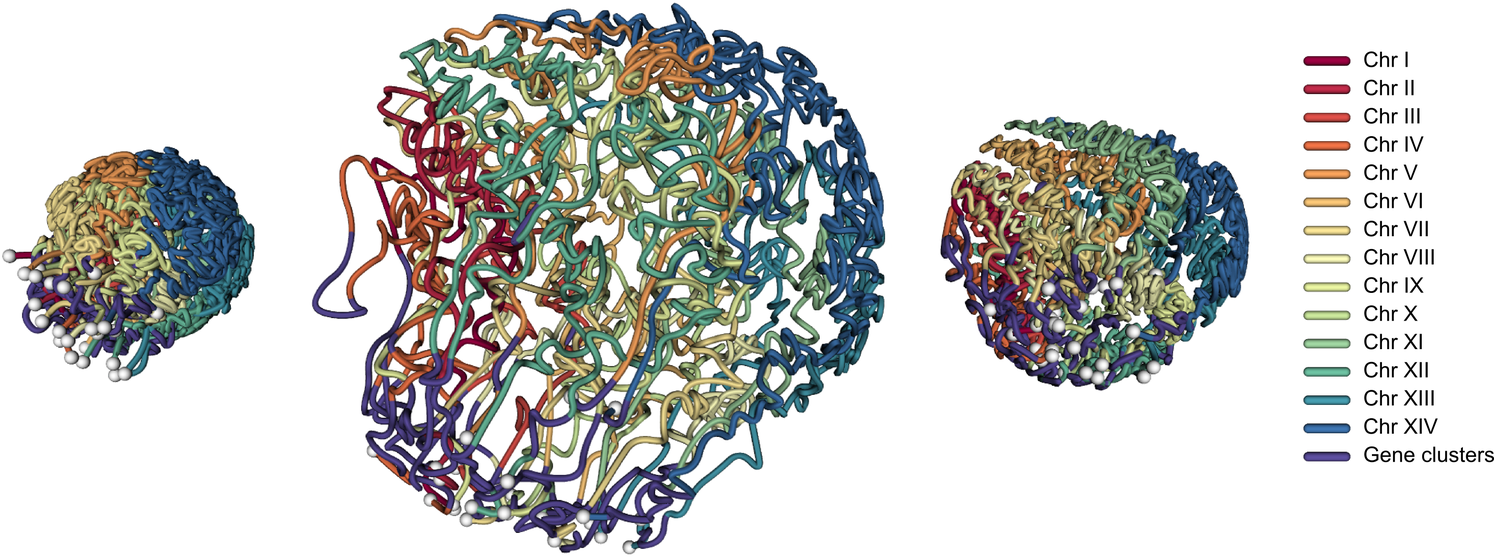
\includegraphics[width=0.95\linewidth]{figures/3D_var_genes.png}
\end{center}

\begin{columns}
\begin{column}{0.15\textwidth}
\bf \small Ring
\end{column}
\begin{column}{0.25\linewidth}
\bf \small Trophozoite
\end{column}
\begin{column}{0.3\linewidth}
\bf \small Schizont
\end{column}
\end{columns}
\end{frame}

% 4. Validation
\begin{frame}
\frametitle{Colocalization of loci is validated with FISH}
\begin{figure}
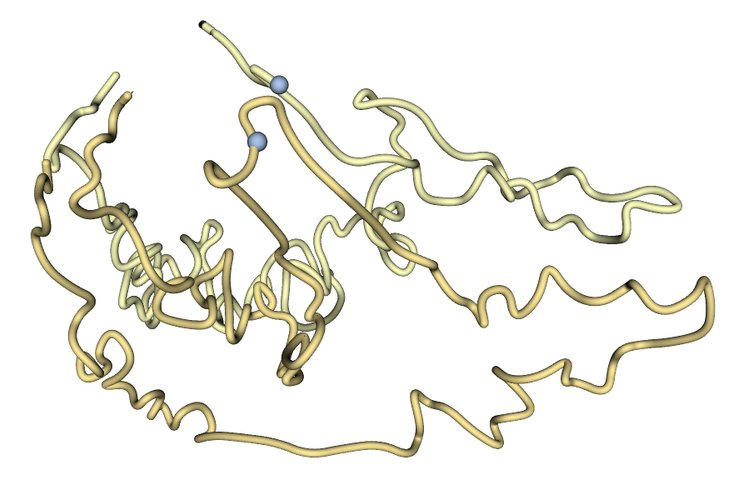
\includegraphics[scale=0.2]{figures/3D_FISH_1.jpg}
\end{figure}
\begin{figure}
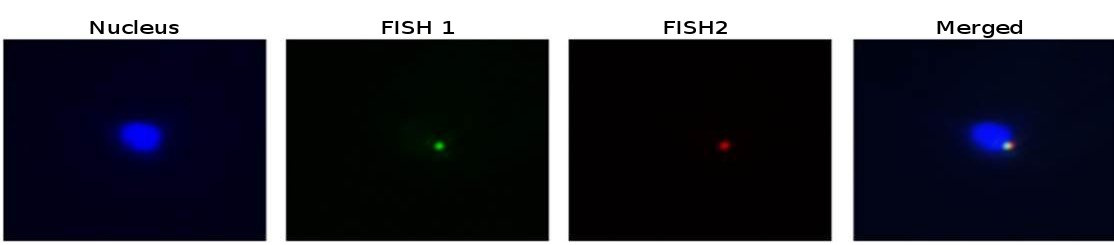
\includegraphics[scale=0.45]{figures/FISH_1.jpg}
\caption{\textbf{Var genes on chromosomes VII and VIII colocolize}
}
\end{figure}
\end{frame}

\begin{frame}
\frametitle{Biological insights on the 3D architecture of the genome}

\begin{itemize}[label={$\bullet$}]

\item Virulence gene clusters on different chromosomes colocalize in 3D.
\item Highly transcribed rDNA units colocalize in 3D during the ring stage.
\item Transcriptionally active trophozoite stage exhibits an open chromatin
structure.
\item VRSM gene clusters form domain-like structures.
\end{itemize}

\begin{center}
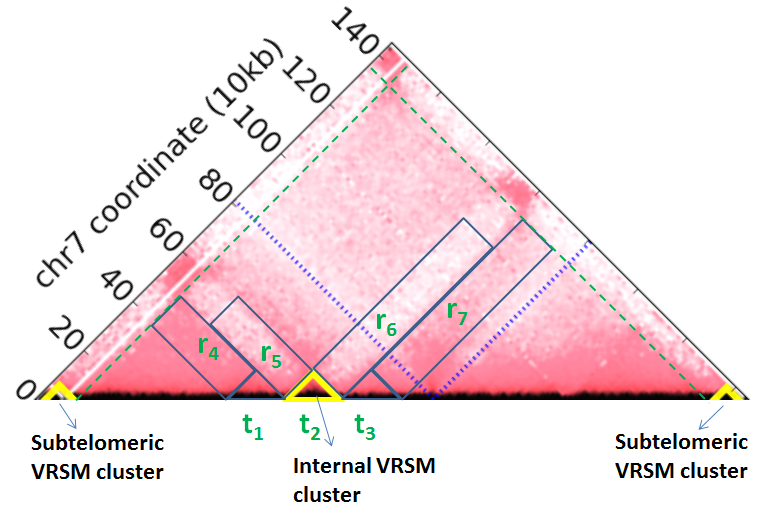
\includegraphics[width=0.5\linewidth]{figures/plasmo_TAD.png}
\end{center}
\end{frame}

% 6. VE modeling

% 6.0 VE modeling results
% 7. Link to gene expression
% 7.0 kernelCCA
\begin{frame}
\frametitle{Identifying links between gene expression profiles and 3D structure}
{\color{Blue} \textbf{Motivation:}} Extract a gene expression profile 
$v \in \mathbb{R}^p$ that is:
\begin{itemize}[label={$\bullet$}]

\item representative of the gene expression profiles ;
\item correlated with the 3D structure;
\end{itemize}
\vspace{1em}
{\color{Blue} \textbf{Data:}}
For each gene $g \in \mathcal{G}$
\begin{itemize}[label={$\bullet$}]
\item Log expression profiles at 27 datapoints: $e(g) = \left( e_1(g), \ldots, e_p(g)\right) \in \mathbb{R}^p$ .
\item Gene's 3D coordinates, extracted from the inferred 3D structure: $x(g)$.
\end{itemize}
\vspace{1em}
{\color{Blue} \textbf{Method}:}
 KernelCCA \citep{vert:graph, bach:kernel}

\end{frame}

\begin{frame}
\frametitle{Extracting a vector $v$ representative of the gene expression
profiles}
Find $v \in \mathbb{R}^p$ to maximize:
\begin{equation*}\label{eq:variance}
V(v) = \frac{\sum_{g \in \mathcal{G}} \left(v^T e(g)\right)^2}{\|v\|^2}\,
\end{equation*}

\begin{figure}
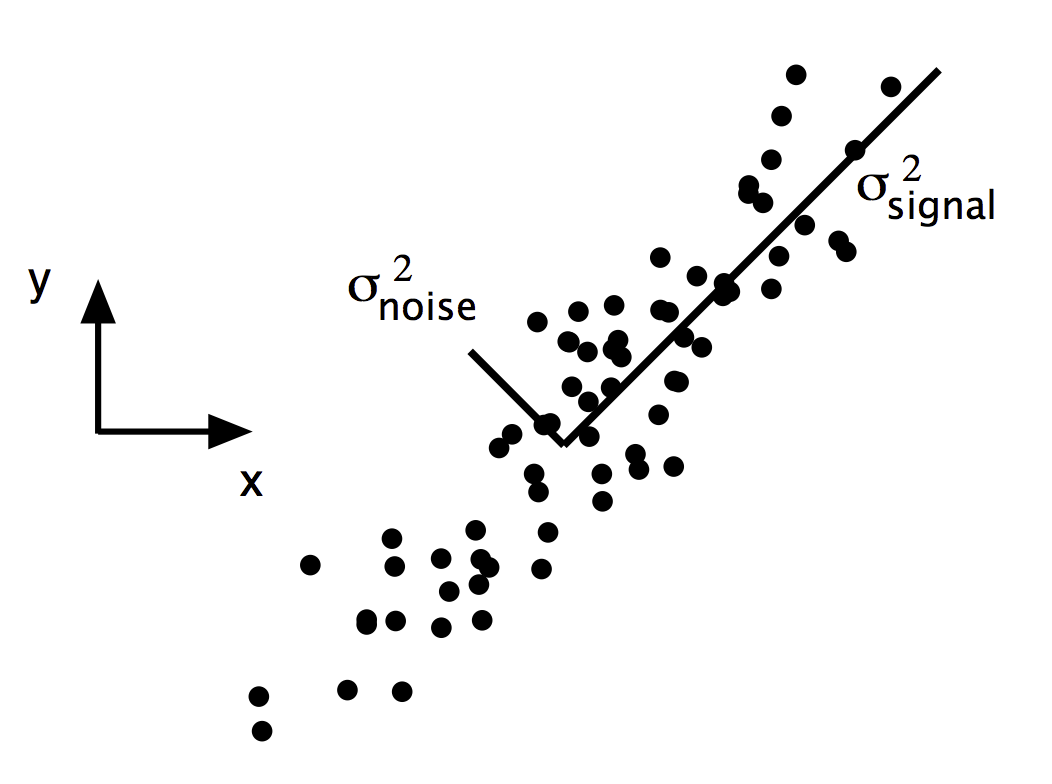
\includegraphics[width=0.5\linewidth]{figures/pca.png}
\end{figure}
\end{frame}

\begin{frame}
\frametitle{Find $f$ such that $f$ is smooth with respect to the 3D structure}
Let $f$ be a vector of scores assigned to each genes. \\
\begin{equation*}\label{eq:smoothness}
S(f) = \frac{f^\top K^{-1}_{3D} f}{||f||^2}\,
\end{equation*}

\vspace{1em}
We want:
\begin{itemize}[label={$\bullet$}]
\item $V(v)$ be large,
\item $S(f)$ be small,
\item $\left(v^\top e(g)\right)_{g\in\mathcal{G}}$ and $f$ be as correlated as possible
\end{itemize}

\vspace{1em}
\begin{center}
{\color{Blue} \bf This can be cast as a generalized eigenvalue problem}
\end{center}

\end{frame}


\begin{frame}
\frametitle{KernelCCA reveals a strong correlation between gene expression
profiles and 3D structure}
\begin{figure}
\begin{center}
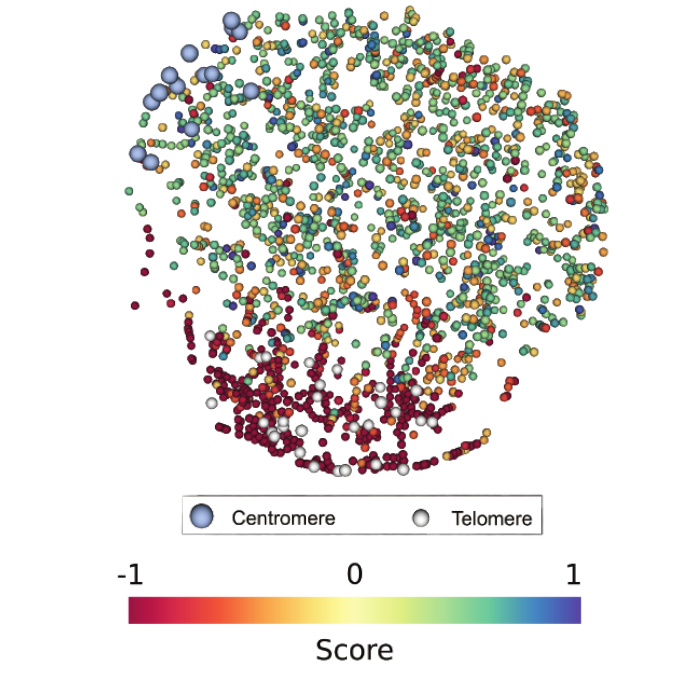
\includegraphics[width=0.6\linewidth]{figures/test.png}
\end{center}
\end{figure}
\end{frame}

% 7.1 results
% 8. Conclusion
\begin{frame}
\frametitle{Conclusion}
\begin{itemize}[label={$\bullet$}]
\item We built high-resolution models of {\em P. falciparum}'s genome
architecture at three time points.
\item We observed :
\begin{itemize}[label={$\bullet$}]
\item strong clustering of centromeres, telomeres, virulance genes
and rDNA, resulting in a {\bf complex architecture}.
\item strong correlation between 3D genome architecture and gene expression.
\end{itemize}
\item {\bf Disruption of the parasite's genome organization} is likely to
interfere with its life cycle, and could therefore be {\bf lethal}.
\end{itemize}

\end{frame}

\section{Accurate identification of centromere location in yeasts using Hi-C}
\begin{frame}
\Large{ \bf
Accurate identification of centromere locations in yeasts using Hi-C.}

\begin{flushright}
\vspace{1em}
\small

\textit{joint work with  Ivan Liachko, Josh Burton, \\
Ferhat Ay, Jay Shendure, Maitreya Dunham, \\ Jean-Philippe Vert and William S.
Noble 
}
\end{flushright}

\end{frame}

% 1. Introduction of the yeasts genome architecture -> Rabl conformation
\begin{frame}
\frametitle{Yeasts are widely studied, widely used organisms}
\only<1>{

\includegraphics[width=0.9\linewidth]{figures/plasmids_without_centromeres_1.eps}
}
\only<2>{
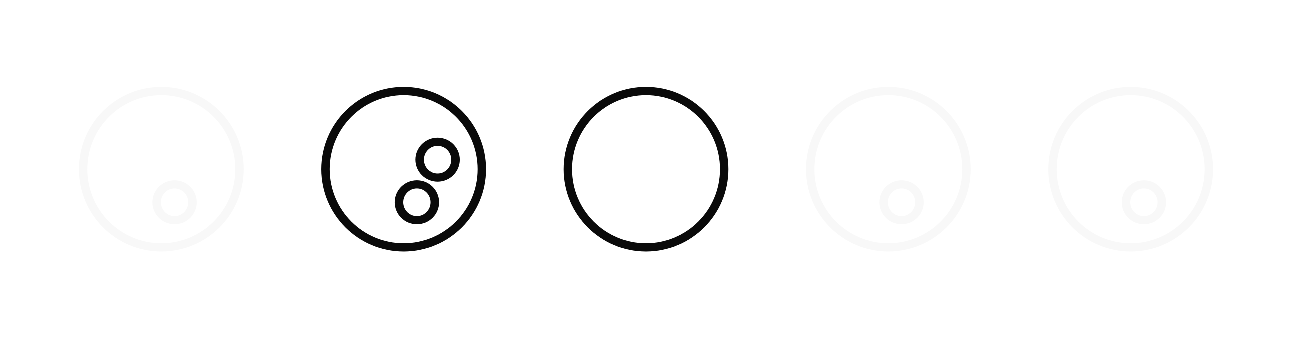
\includegraphics[width=0.9\linewidth]{figures/plasmids_without_centromeres_2.eps}
}
\only<3>{
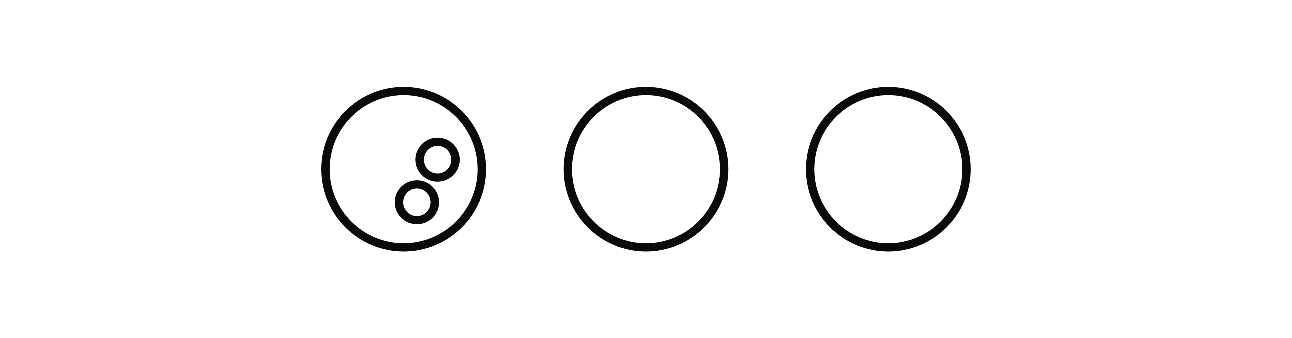
\includegraphics[width=0.9\linewidth]{figures/plasmids_without_centromeres_3.eps}
}
\only<4>{
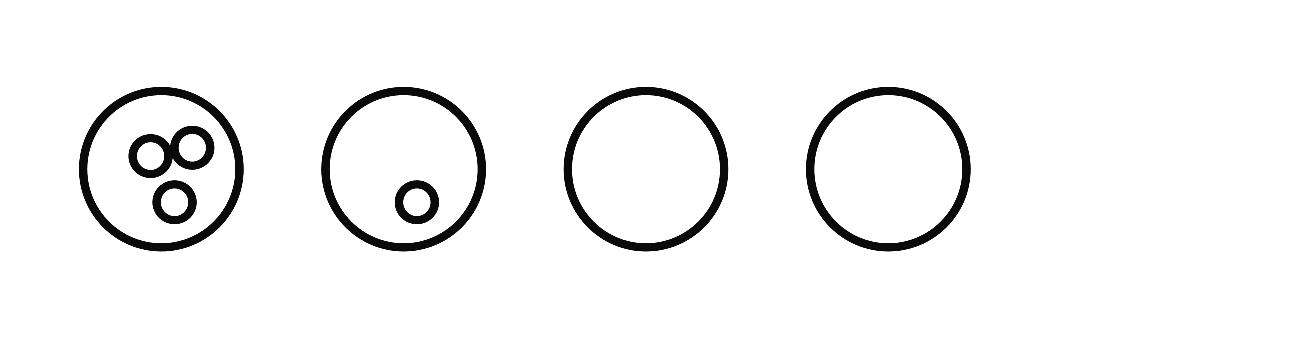
\includegraphics[width=0.9\linewidth]{figures/plasmids_without_centromeres_4.eps}
}
\only<5>{
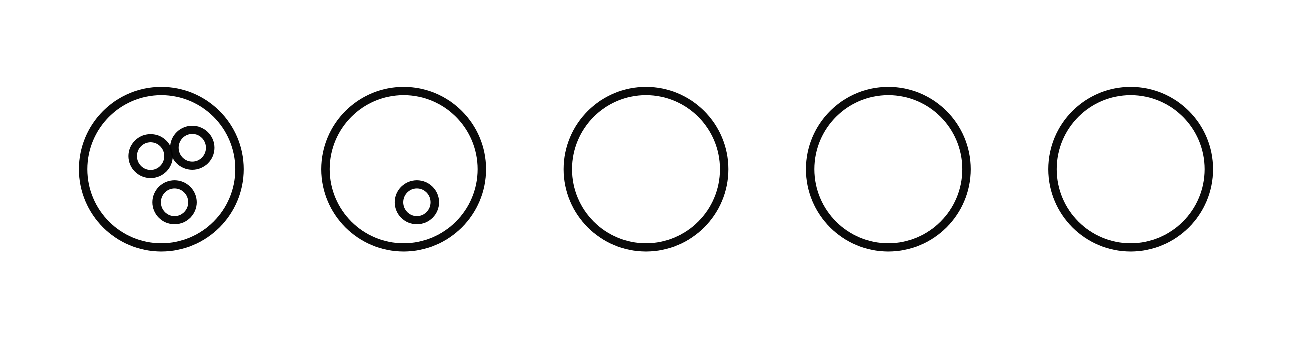
\includegraphics[width=0.9\linewidth]{figures/plasmids_without_centromeres_5.eps}
}
\only<6>{
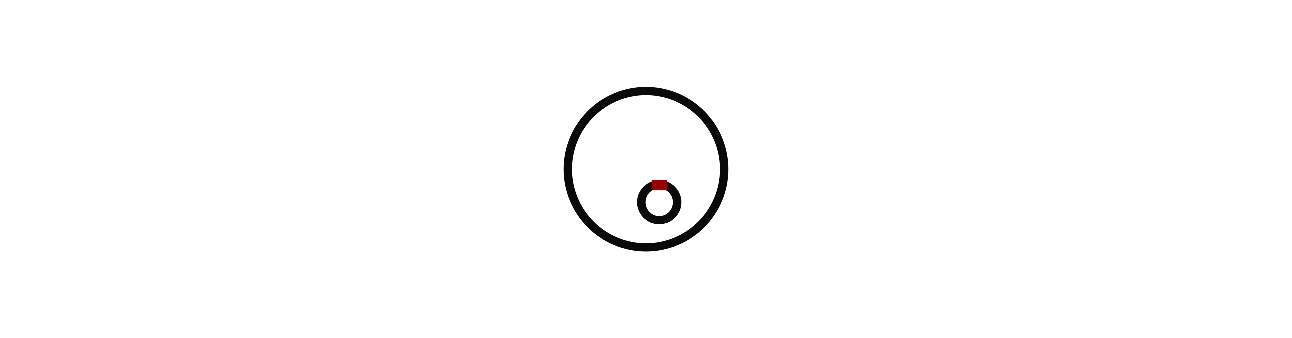
\includegraphics[width=0.9\linewidth]{figures/plasmids_with_centromeres_1.eps}
}
\only<7>{
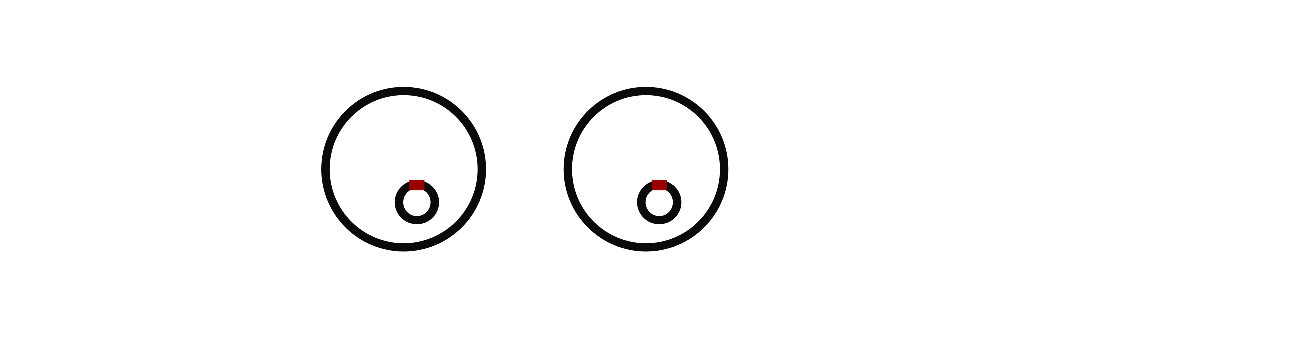
\includegraphics[width=0.9\linewidth]{figures/plasmids_with_centromeres_2.eps}
}
\only<8>{
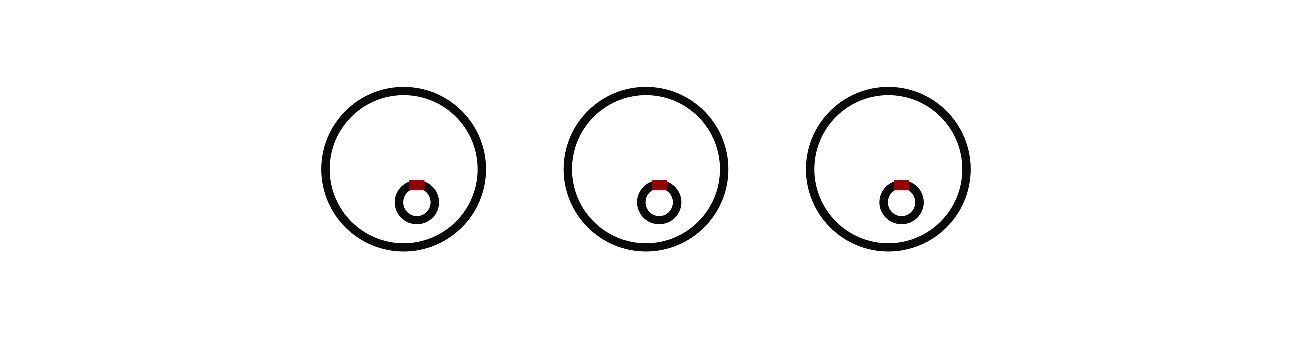
\includegraphics[width=0.9\linewidth]{figures/plasmids_with_centromeres_3.eps}
}
\only<9>{
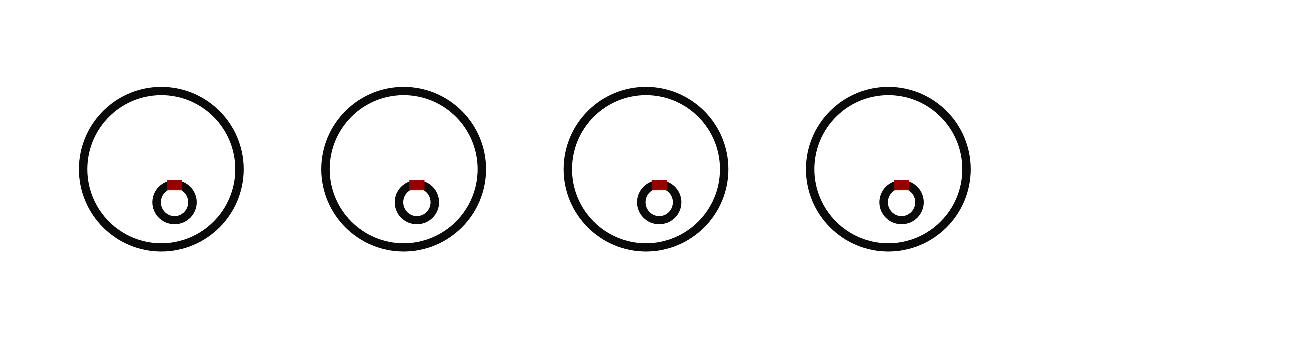
\includegraphics[width=0.9\linewidth]{figures/plasmids_with_centromeres_4.eps}
}
\only<10>{
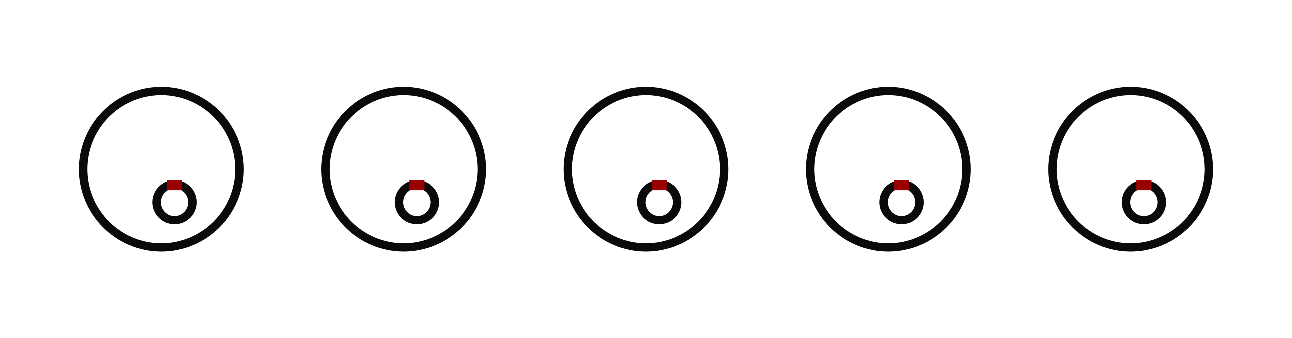
\includegraphics[width=0.9\linewidth]{figures/plasmids_with_centromeres_5.eps}
}

{\color{Blue} \textbf{Motivation}}
\begin{itemize}
\item Yeasts are crucial organisms in biotechnology applications.
\item Centromeres allow proper segregation of chromosomes.
\end{itemize}

\vspace{1em}
{\color{Blue} \textbf{Goal}} Develop a robust and accurate method to detect
centromere locations in yeasts.

\vspace{1em}
{\color{Blue} \textbf{Idea}} Leverage the yeasts' genome architecture (where
centromeres colocalize) and Hi-C
data to detect centromere locations.
\end{frame}

% 2. Motivation
\begin{frame}
\frametitle{Yeasts' centromeres colocalize in the nucleus}
\begin{figure}
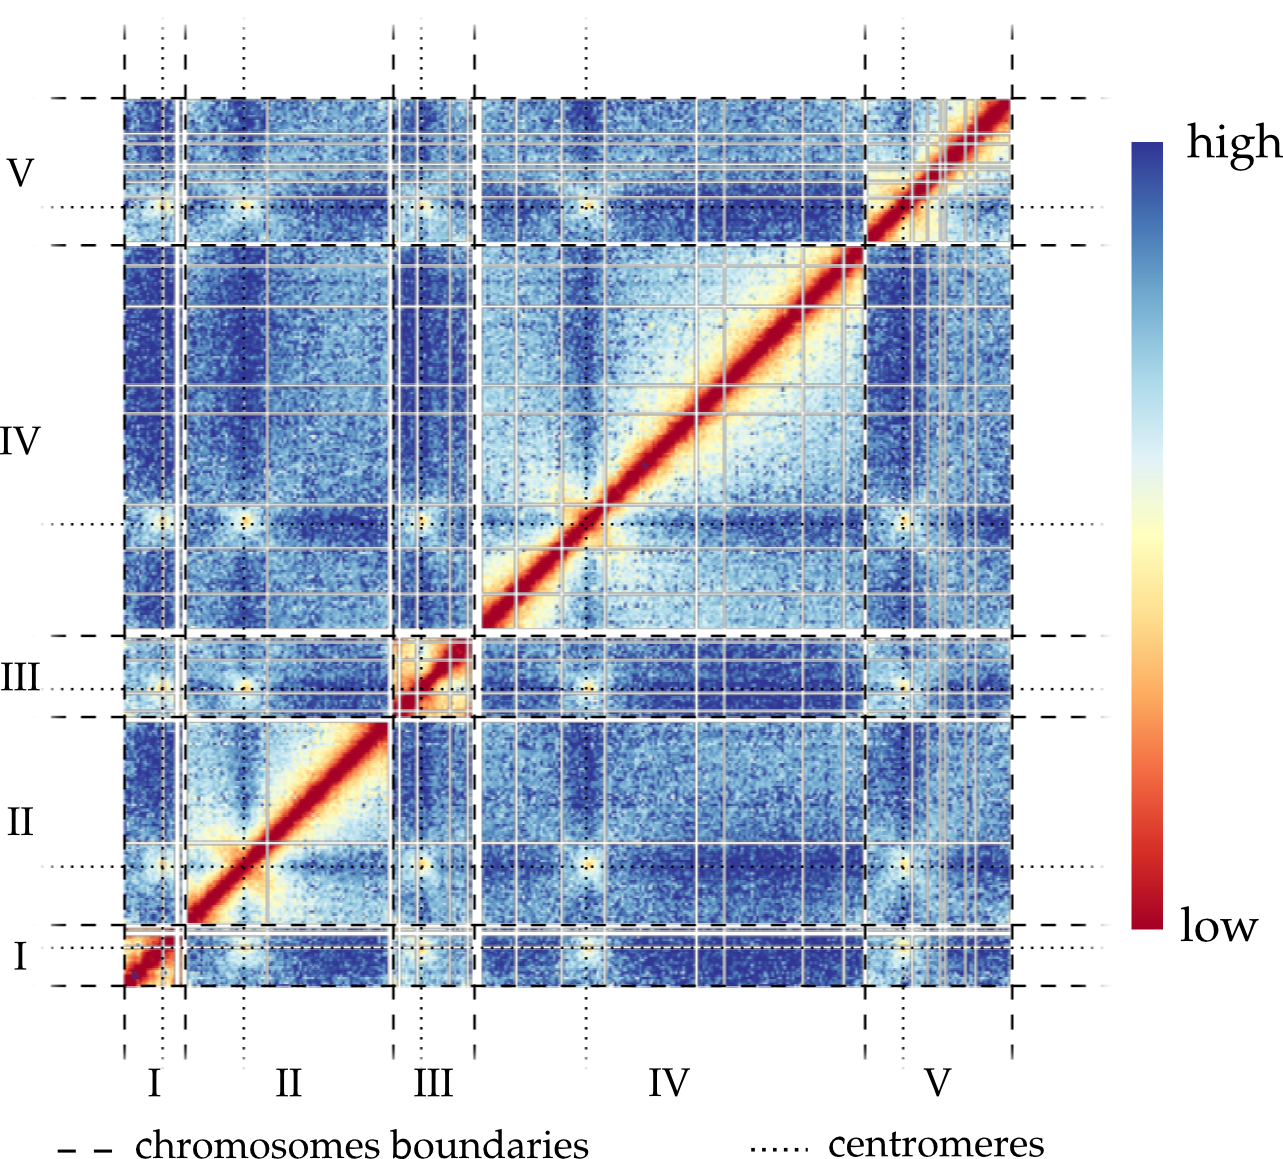
\includegraphics[width=0.52\textwidth]{figures/yeast_counts.pdf}
\caption{Contact counts for the first 5 chromosomes of \textit{S. cerevisiae}}
\end{figure}
\end{frame}

\begin{frame}
\frametitle{Centurion in brief}
\begin{figure}
\includegraphics[width=0.85\textwidth]{figures/centurion_brief.pdf}
\end{figure}
\end{frame}

% 3. Idea
\begin{frame}
\frametitle{Contact enrichment as a Gaussian function}
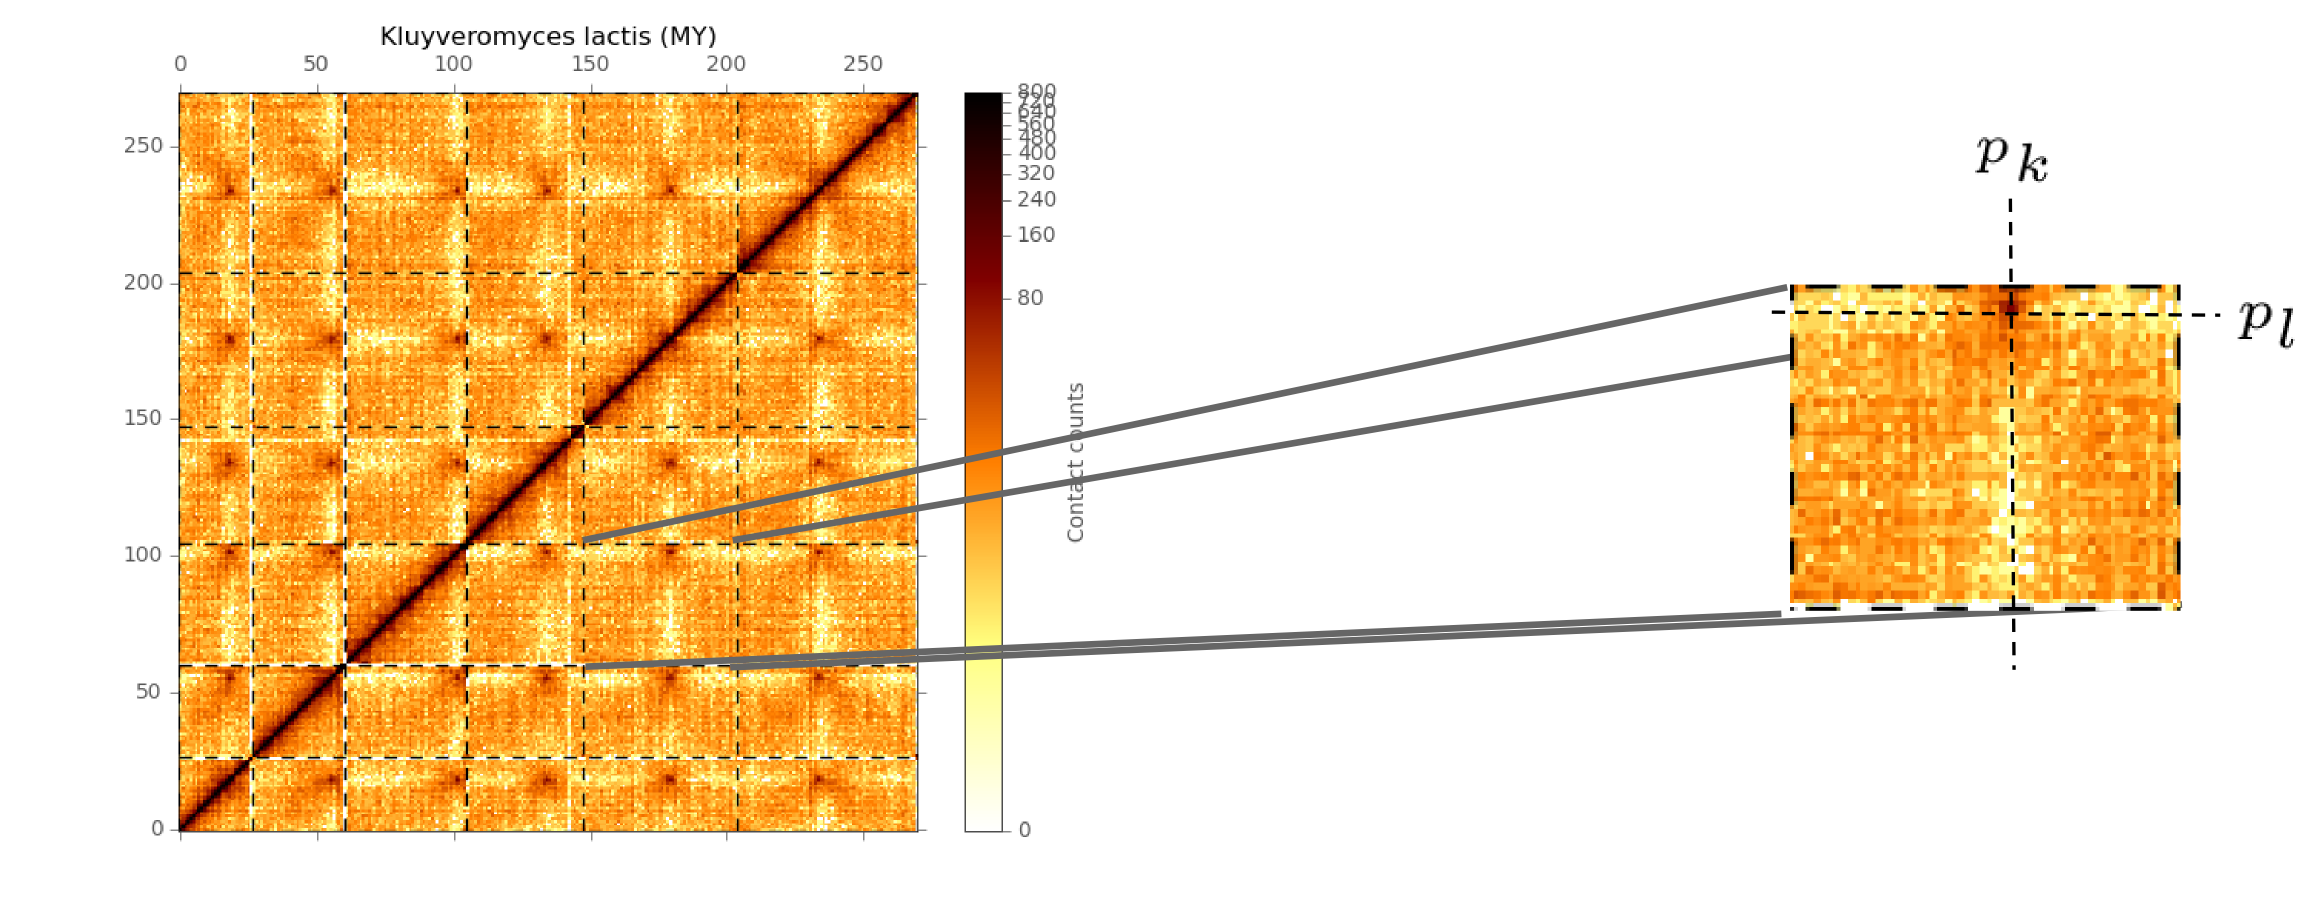
\includegraphics[width=\linewidth]{figures/centurion_idea.png}
\begin{flushright}
$a\exp \left(- \frac{(x_i -
p_k)^2 + (x_j - p_l)^2)}{2\sigma^2}\right)$
\end{flushright}
\end{frame}

% 4. Optimization problem
\begin{frame}
\frametitle{Centromere detection as an optimization problem}

\begin{equation*}
\renewcommand{\arraystretch}{2}
\begin{array}{ccll}
\underset{\textbf{P}, a, \sigma, b}{\text{minimize}} & &
\sum_{(i,j)\in\mathcal{D}} \left[ c_{ij} - a\exp \left(- \frac{(x_i -
p_{B(i)})^2 + (x_j - p_{B(j)})^2)}{2\sigma^2}\right) - b \right]^2\,. \\
\text{subject to} & & p_i\quad\text{belongs to chromosome }i
\end{array}
\end{equation*}

where
\begin{itemize}[label={$\bullet$}]
\item $B(i)$ is a mapping between locus $i$ and its chromosome.
\item $p_{B(i)}$ corresponds to the centromere candidate of locus $i$'s
chromosome.
\end{itemize}
\end{frame}

\begin{frame}
\frametitle{Initializing the optimization problem}

{\color{Blue} \bf Problems}
\begin{itemize}[label={$\bullet$}]
\item The objective function is non convex.
\item Other DNA regions colocolize and highly interact with one another.
\end{itemize}

\vspace{1em}
{\color{Blue} \bf Solutions}
\begin{itemize}[label={$\bullet$}]
\item Use the inter chromosomal contact counts enrichments to identify
potential candidates (typically two per chromosomes).
\item Initialize the optimization with all possible combinations.
\end{itemize}

\end{frame}

% 5. Initialization
% 6. Results
\begin{frame}
\frametitle{Centromeres' call on \textit{S. cerevisiae}}
\begin{figure}
\includegraphics[width=0.9\linewidth]{figures/2_whole_genome_SC.pdf}
\end{figure}
\end{frame}


\begin{frame}
\frametitle{Centurion accurately predicts centromere locations}
\begin{figure}
\includegraphics[width=0.9\linewidth]{figures/2_pf_zoomed_in.pdf}
\caption{Centromere calling on \textit{P. falciparum}}
\end{figure}
\end{frame}

\begin{frame}
\frametitle{The \citet{marie-nelly:filling} method for centromere detection}

\citet{marie-nelly:filling} propose a two-step method:
\vspace{2em}

\begin{columns}
\begin{column}{0.5\textwidth}
\textbf{1. Prelocalizing centromeres}
\end{column}
\begin{column}{0.5\textwidth}
\textbf{2. Refining the prediction}
\end{column}
\end{columns}

\begin{columns}
\centering
\begin{column}{0.5\textwidth}
\begin{center}
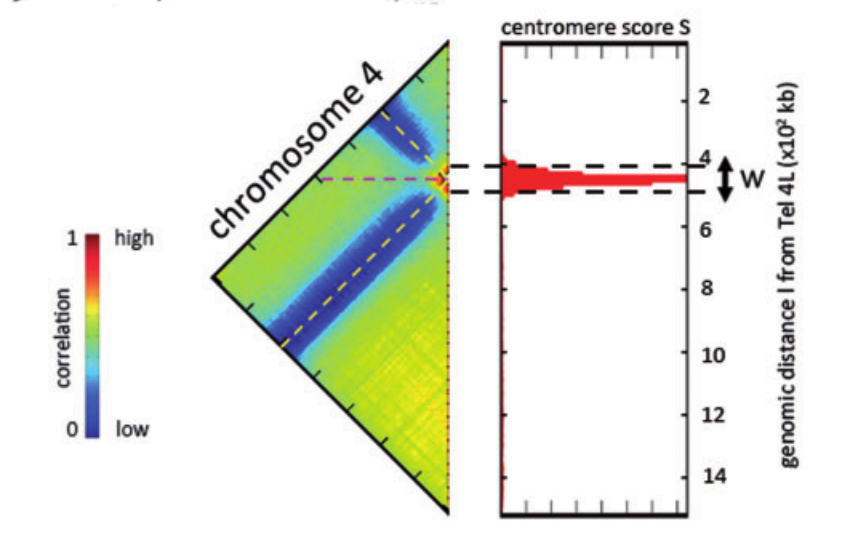
\includegraphics[width=0.75\textwidth]{figures/marie_nelly_prelocation.png}
\end{center}
\end{column}
\begin{column}{0.5\textwidth}
\begin{center}
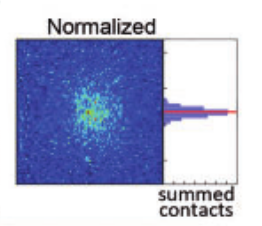
\includegraphics[width=0.5\textwidth]{figures/marie_nelly_step2.png}
\end{center}
\end{column}
\end{columns}

\end{frame}

\begin{frame}
\frametitle{Comparison of the objective functions}

\begin{figure}
\includegraphics[width=0.9\linewidth]{figures/2_MN_vs_us_starting_gt_HR_40000.pdf}
\end{figure}
\end{frame}

\begin{frame}
\frametitle{De novo centromere calls on 6 yeast species}

\textit{K. wickerhamii}, \textit{P. pastoris}, \textit{S. paradoxus}, \textit{L.
waltii}, \textit{E. gossypii}, \textit{S. stipitis}

\begin{figure}
\includegraphics[width=0.9\linewidth]{figures/4_whole_genome_KW.pdf}

\caption{\textbf{\textit{K. wickerhamii}}}
\end{figure}

\end{frame}

\begin{frame}
\frametitle{Conclusion}
\begin{itemize}[label={$\bullet$}]
\item We propose a method called {\bf Centurion} that jointly infers
centromere locations.
\item Centurion predicts accurate centromere locations and outperforms
existing methods, in particular in high noise settings.
\end{itemize}
\end{frame}

% 7. Conclusion

\section{Conclusion and Perspectives}
\begin{frame}
\begin{center}
\huge{ \bf
Conclusion and Perspectives
}
\end{center}
\end{frame}

% 1. Conclusion

\begin{frame}
\frametitle{Conclusion}
\begin{itemize}[label={$\bullet$}]
\item \textbf{Biological contributions} I
studied the 3D structure of {\em P. falciparum}, which led to a \textit{better
understanding of links between the genome architecture and gene expression and
regulation}.
\item \textbf{\em Methodological contributions}
\begin{itemize}[label={$\bullet$}]
\item development of a stable statistical method for \textit{3D genome
inference}
\item robust and accurate algorithm for \textit{centromere detection in yeast} 
\end{itemize}
\item \textbf{\em Software contributions}: 
\begin{itemize}[label={$\bullet$}]
\item scikit-learn, a machine-learning toolkit written in Python
\item PASTIS
\item Centurion
\item iced, included in HiC-pro
\end{itemize}
\end{itemize}
\end{frame}

\begin{frame}
\frametitle{Perspective 1: Inferring models of diploid (or polyploid) genomes.}
\begin{figure}
\centering
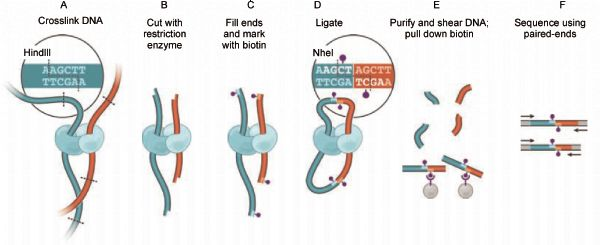
\includegraphics[width=0.85\textwidth]{figures/hic_protocol.jpg}
\caption{\textbf{Hi-C protocol doesn't distinguish between homologous
chromosomes} \citep{rao:3d}}
\end{figure}
\end{frame}



\begin{frame}
\frametitle{Perspective 1: Inferring models of diploid (or polyploid) genomes.}
{\color{Blue} Each entry of the matrix is the sum of contact counts of diploid
homologous chromosomes.}

\begin{figure}
\begin{center}

\includegraphics[width=0.7\linewidth]{figures_/counts_duplicated.pdf}
\end{center}
\end{figure}

\end{frame}

\begin{frame}
\frametitle{Perspective 1: Inferring models of diploid (or polyploid) genomes}

Let
$\Phi:[1,n] \rightarrow [1, m]$ the mapping that associates bead $l$ with loci
$i$.

\begin{equation*}
c_{ij} \sim Poisson(\sum_{\Phi(k) = i, \Phi(l) = j} \beta d_{kl}^{\alpha}) 
\end{equation*}

\begin{figure}
\begin{center}
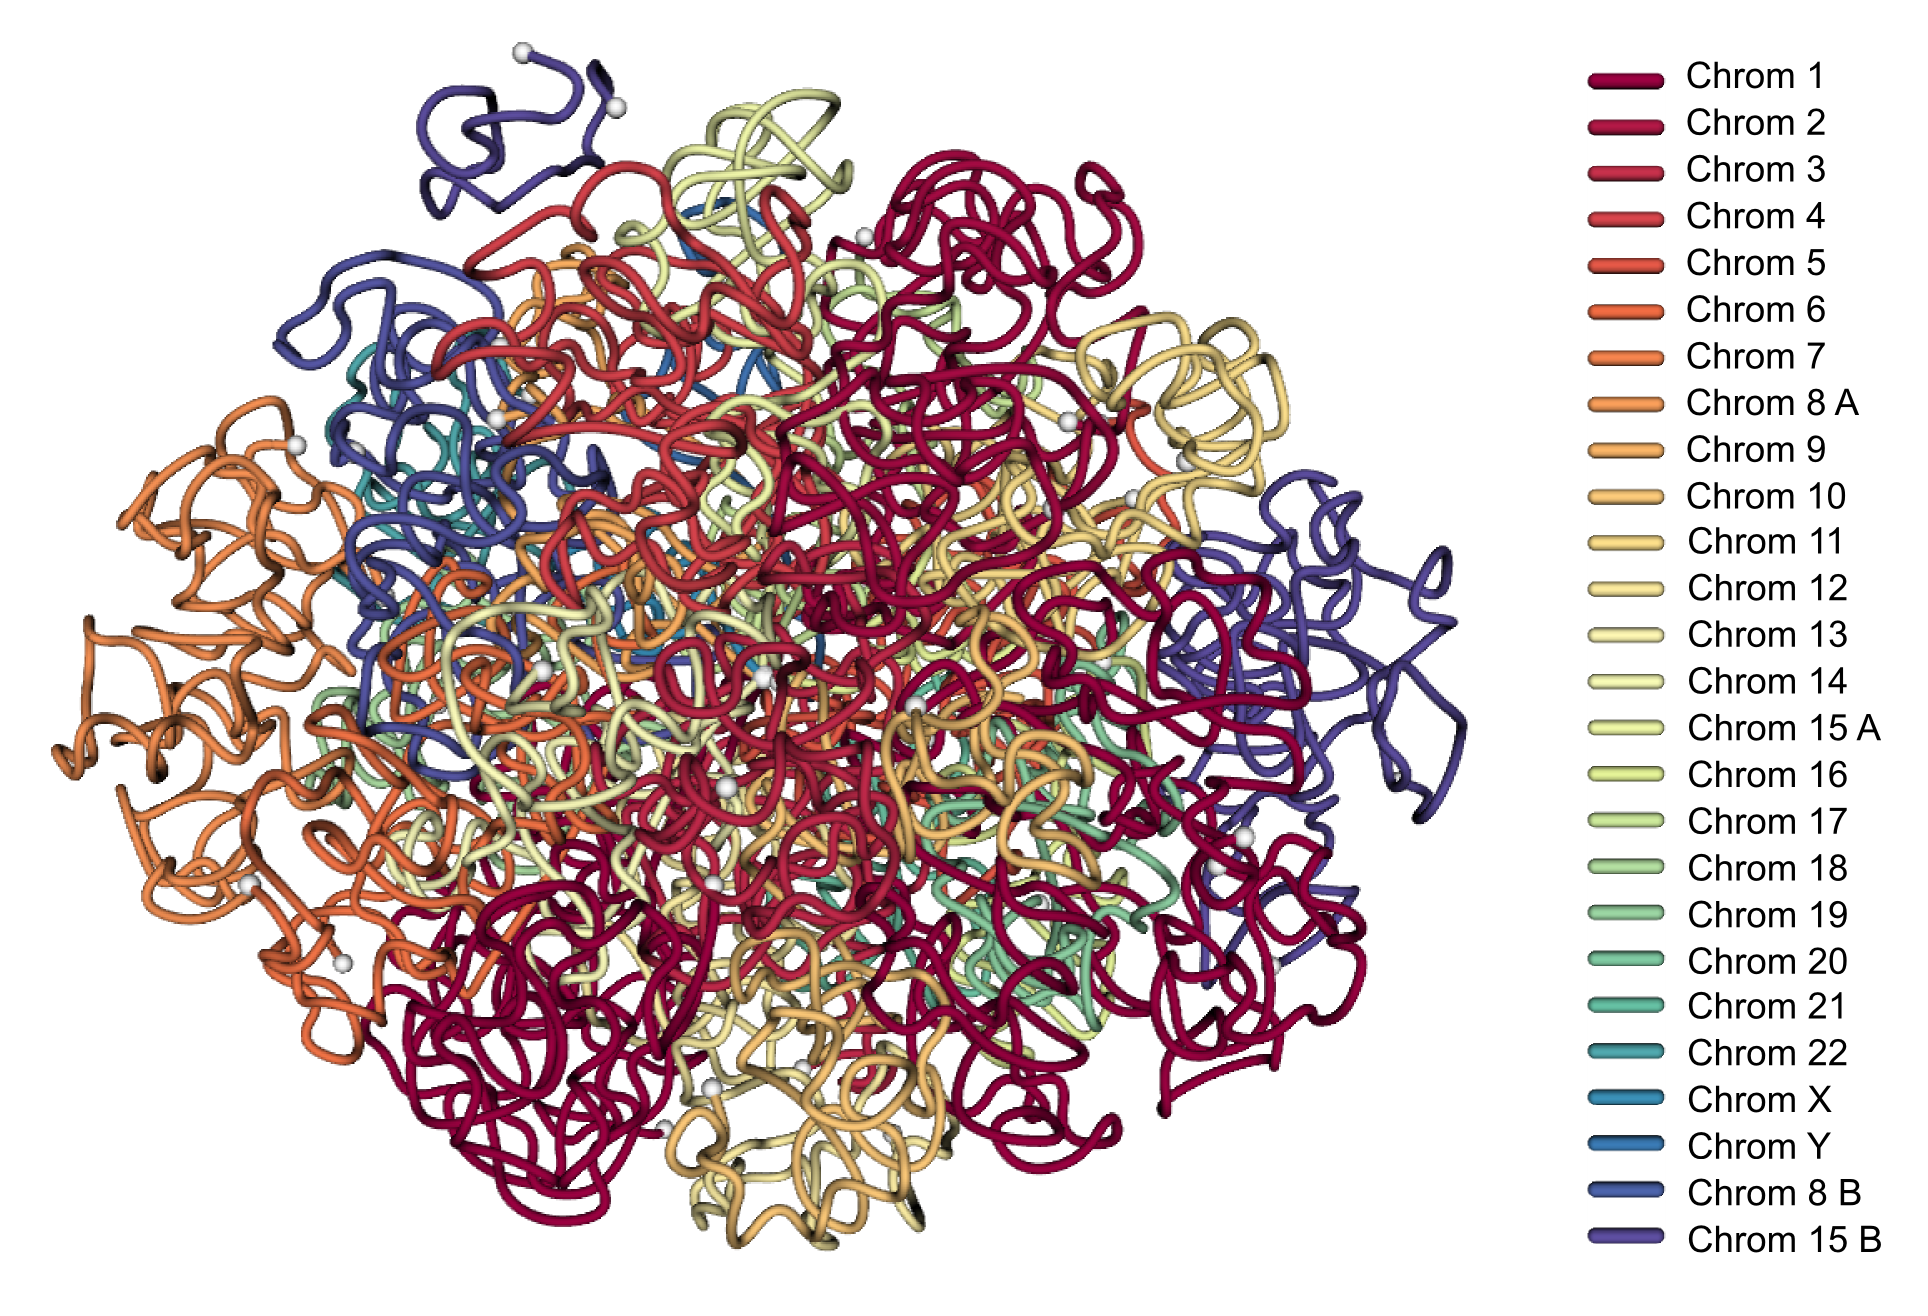
\includegraphics[width=0.6\linewidth]{images_/all_with_legend.png}
\end{center}
\caption{Three-dimensional structure of the KBM7 genome,
which is haploid for all chromosomes other than diploid chromosome 8 (8A, 8B)
and partially diploid chromosome 15 (15A, 15B). Different colors represent
different
chromosomes, and white balls represent chromosome ends}
\end{figure}
\end{frame}

\begin{frame}
\frametitle{Perspective 2: Inferring a population of structures}

Now assume Hi-C data can be summarized by a mixture of $K$ structures
$\mathbf{X}^{(k)}$.

\begin{equation*}
c_{ij} \sim Poisson(\sum_{k}^{K} \gamma_k \beta d^{(k)\alpha}_{ij}) 
\end{equation*}

Each structure $\mathbf{X}^{(k)}$ can be constrained using single cell Hi-C.

\begin{figure}
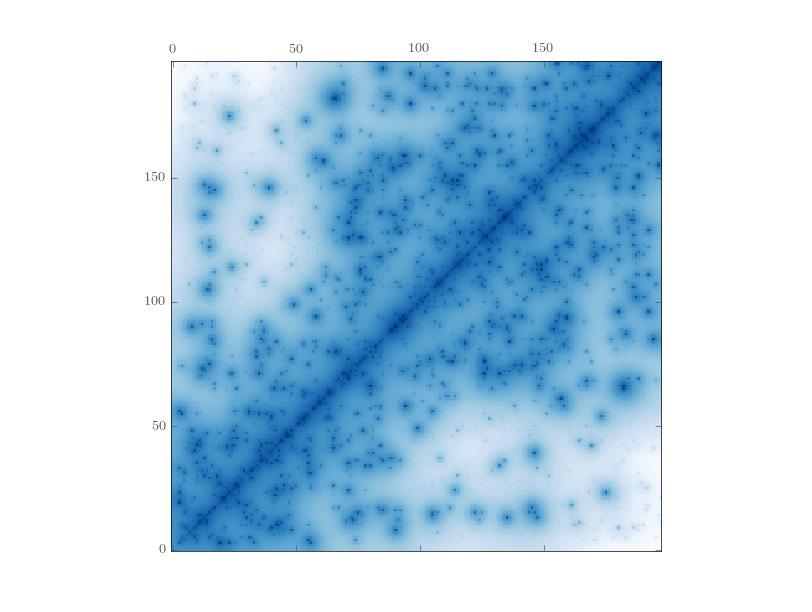
\includegraphics[width=0.4\linewidth]{figures_/chr1_cell5.png}
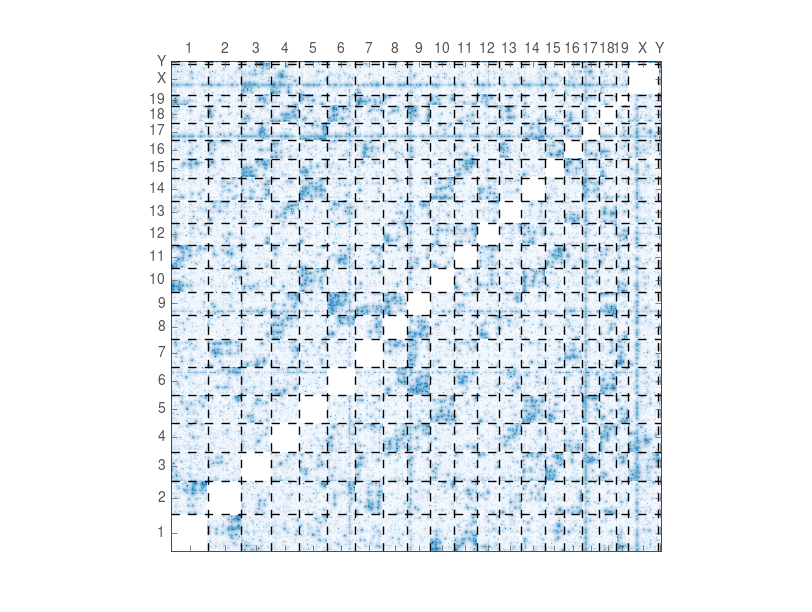
\includegraphics[width=0.4\linewidth]{figures_/all_chr_cell5.png}
\caption{Single cell Hi-C - cell 5 \citep{nagano:single-cell}}
\end{figure}
\end{frame}

\begin{frame}
\frametitle{Perspective 3: Inferring genome 3D architecture by modeling
overdispersion of Hi-C data}

{\bf \color{Blue} Motivation} Current methods for inferring 3D models of genome
architecture fail on noisy datasets.

\vspace{1em}
{\bf \color{Blue} Why} \texttt{Pastis} models contact counts as Poisson random variables,
which is {\color {Blue}} not suited for overdispersed data.

\vspace{1em}
{\bf \color{Blue} Idea} use the Negative Binomial distribution to better
model overdispersion.

\begin{figure}
\includegraphics[width=0.5\linewidth]{figures_/SPZ_pf_MDS_vs_NBcst0.pdf}
\end{figure}
\end{frame}



% 2. Acknowledgments
\begin{frame}
\frametitle{Acknowledgments}
\fboxsep=0pt
\noindent
\begin{minipage}[t]{0.48\linewidth}
\textbf{Mines ParisTech - CBIO} \\
Jean-Philippe \textsc{Vert} \\
Thomas \textsc{Walter} \\
V\'eronique \textsc{Stoven} \\

\textbf{UW - Noble lab} \\
William S. \textsc{Noble} \\
Ferhat \textsc{Ay} \\
Kate \textsc{Cook} \\
Gurkan \textsc{Yardimci} \\

\textbf{Institut Curie - U900} \\
Emmanuel \textsc{Barillot} \\
Nicolas \textsc{Servant} \\
Chong-Jian \textsc{Chen} \\
Eric \textsc{Viara} \\


\end{minipage}
\hfill%
\begin{minipage}[t]{0.48\linewidth}

\small
\textbf{UC Riverside} \\
Karine \textsc{Le Roch} \\
Sebastiaan \textsc{Bol} \\
Evelien \textsc{Bunnik} \\
Jacques \textsc{Prudhomme} \\

\textbf{UMass} \\
Job \textsc{Dekker} \\
Bryan \textsc{Lajoie} \\


\textbf{Institut Curie - UMR168} \\
Edith \textsc{Heard} \\

\textbf{UW - Dunham lab} \\
Maitreya \textsc{Dunham} \\
Ivan \textsc{Liachko} \\

\textbf{UW - Shendure lab} \\
Jay \textsc{Shendure} \\
Josh \textsc{Burton} \\

\end{minipage}

\end{frame}

\begin{frame}[allowframebreaks,noframenumbering]
  \frametitle{References}
  \bibliographystyle{plainnat}
  \bibliography{refs}
\end{frame}

\begin{frame}[noframenumbering]

\end{frame}

\begin{frame}[noframenumbering]
\frametitle{GSEA shows strong enrichments of GO terms in telomeric and
non-telomeric regions}

\begin{table}
\footnotesize
\vspace{10pt}
\begin{center}
\begin{tabular}{lp{0.4\linewidth}ccc}
\hline
\emph{GO term }&  \emph{Description} & \emph{Type} & \emph{Enrichment} &
\emph{q-value}  \\
\hline
GO:0005840 & ribosome & CC & n-t & 0.000\\
GO:0005622 & intracellular & CC & n-t & 0.000\\
GO:0022627 & cytosolic small ribosomal subunit & CC & n-t & 0.000\\
GO:0005789 & endoplasmic reticulum membrane & CC & n-t & 0.000\\
GO:0005783 & endoplasmic reticulum & CC & n-t & 0.000\\
GO:0022625 & cytosolic large ribosomal subunit & CC & n-t & 0.000\\
GO:0015935 & small ribosomal subunit & CC & n-t & 0.000\\
GO:0020002 & host cell plasma membrane & CC & t & 0.000\\
GO:0020030 & infected host cell surface knob & CC & t & 0.000\\
GO:0020036 & Maurer's cleft & CC & t & 0.000\\
GO:0016021 & integral to membrane & CC & t & 0.000\\
GO:0015934 & large ribosomal subunit & CC & n-t & 0.001\\
\dots & \dots & \dots & \dots & \dots \\
\end{tabular}
\end{center}
\end{table}
\end{frame}



\end{document}

